\fenicschapter{Computational hemodynamics}
              {Computational hemodynamics}
              {Computational hemodynamics}
              {Kristian Valen-Sendstad, Kent-Andre Mardal and Anders Logg}
              {kvs-2}

\index{hemodynamics}

Computational fluid dynamics (CFD) is a tool with great potential in
medicine. Using traditional engineering techniques, one may compute,
e.g., the blood flow in arteries and the resulting stress on the
vessel wall to understand, treat and prevent various cardiovascular
diseases. This chapter is devoted to the computation of blood flow in
large cerebral arteries and how the blood flow affects the development
and rupture of aneurysms. We discuss the process, from generating
geometries from medical imaging data to performing patient-specific
simulations of hemodynamics in FEniCS. Specifically, we present three
different applications: simulations related to a recently published
study by~\citet{LindekleivValen-SendstadMorganEtAl2010} concerning
gender differences in cerebral arteries, a study of the carotid
arteries of a canine with an induced aneurysm described
in~\citet{JiangJohnsonValen-SendstadEtAl2010}, and a study of the
blood flow in a healthy Circle of Willis, where patient-specific
velocity measurements are compared with a model for the peripheral
resistance.

%------------------------------------------------------------------------------
\section{Medical background} \label{Medical_Background}

Stroke is a leading cause of death in the developed part of the
world \citep{Feigin2005}, and mortality rates could increase
dramatically in the years to come \citep{MurrayLopez1997}. Stroke is
caused by an insufficient supply of blood to parts of the brain. There
are mainly two different types of strokes: ischemia caused by
obstructions in the blood vessels, and subarachnoid hemorrhage caused
by the rupture of one or more aneurysms. Aneurysms typically develop
in or near the so-called Circle of Willis, which is an arterial
network of vessels at the base of the brain. The function of this
circle is believed to be to ensure a robust and redundant system in
the sense that the brain receives a sufficient amount of blood even if
one of the vessels is occluded or under-developed. This network
connects the internal carotid arteries (ICA) and the vertebral
arteries (VA) in a circle-like structure, and it is the main
supplier of blood to the brain. Figure~\ref{fig:kvs-2:textbook-circle}
shows the circle as typically depicted in textbooks. Blood enters the
circle through the ICAs, which are located at the front of the neck,
and the VAs located in the back of the neck.  The VAs join in the
Basilar Artery (BA), and blood leaves the circle in the front through
the Anterior Cerebral Arteries (ACA), in the back through the
Posterior Cerebral Arteries (PCA), and at the sides through the Middle
Cerebral Arteries (MCA). A patient-specific circle, the one used in
Section~\ref{cok}, is shown in Figure~\ref{fig:kvs-2:circle_kent}.

% Figure from old book (Gray's anatomy) which has expired Copyright,
% copied from wikipedia: http://en.wikipedia.org/wiki/Circle_of_Willis
\begin{figure}
  \centering
  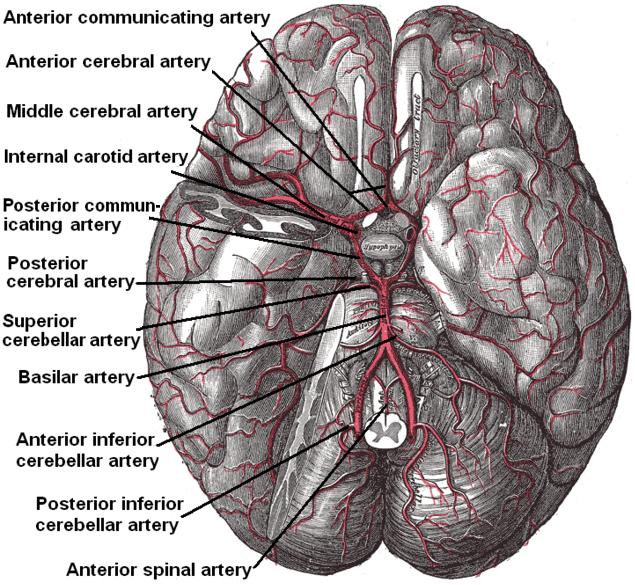
\includegraphics[width=\largefig]{chapters/kvs-2/png/cow_gray_1.png} \\
  \caption{Illustration of the Circle of Willis and the base of the brain
      seen from beneath. The illustration is taken from Gray's Anatomy~\citep{Gray1897}.}
  \label{fig:kvs-2:textbook-circle}
\end{figure}

\begin{figure}
\bwfig
  \centering
  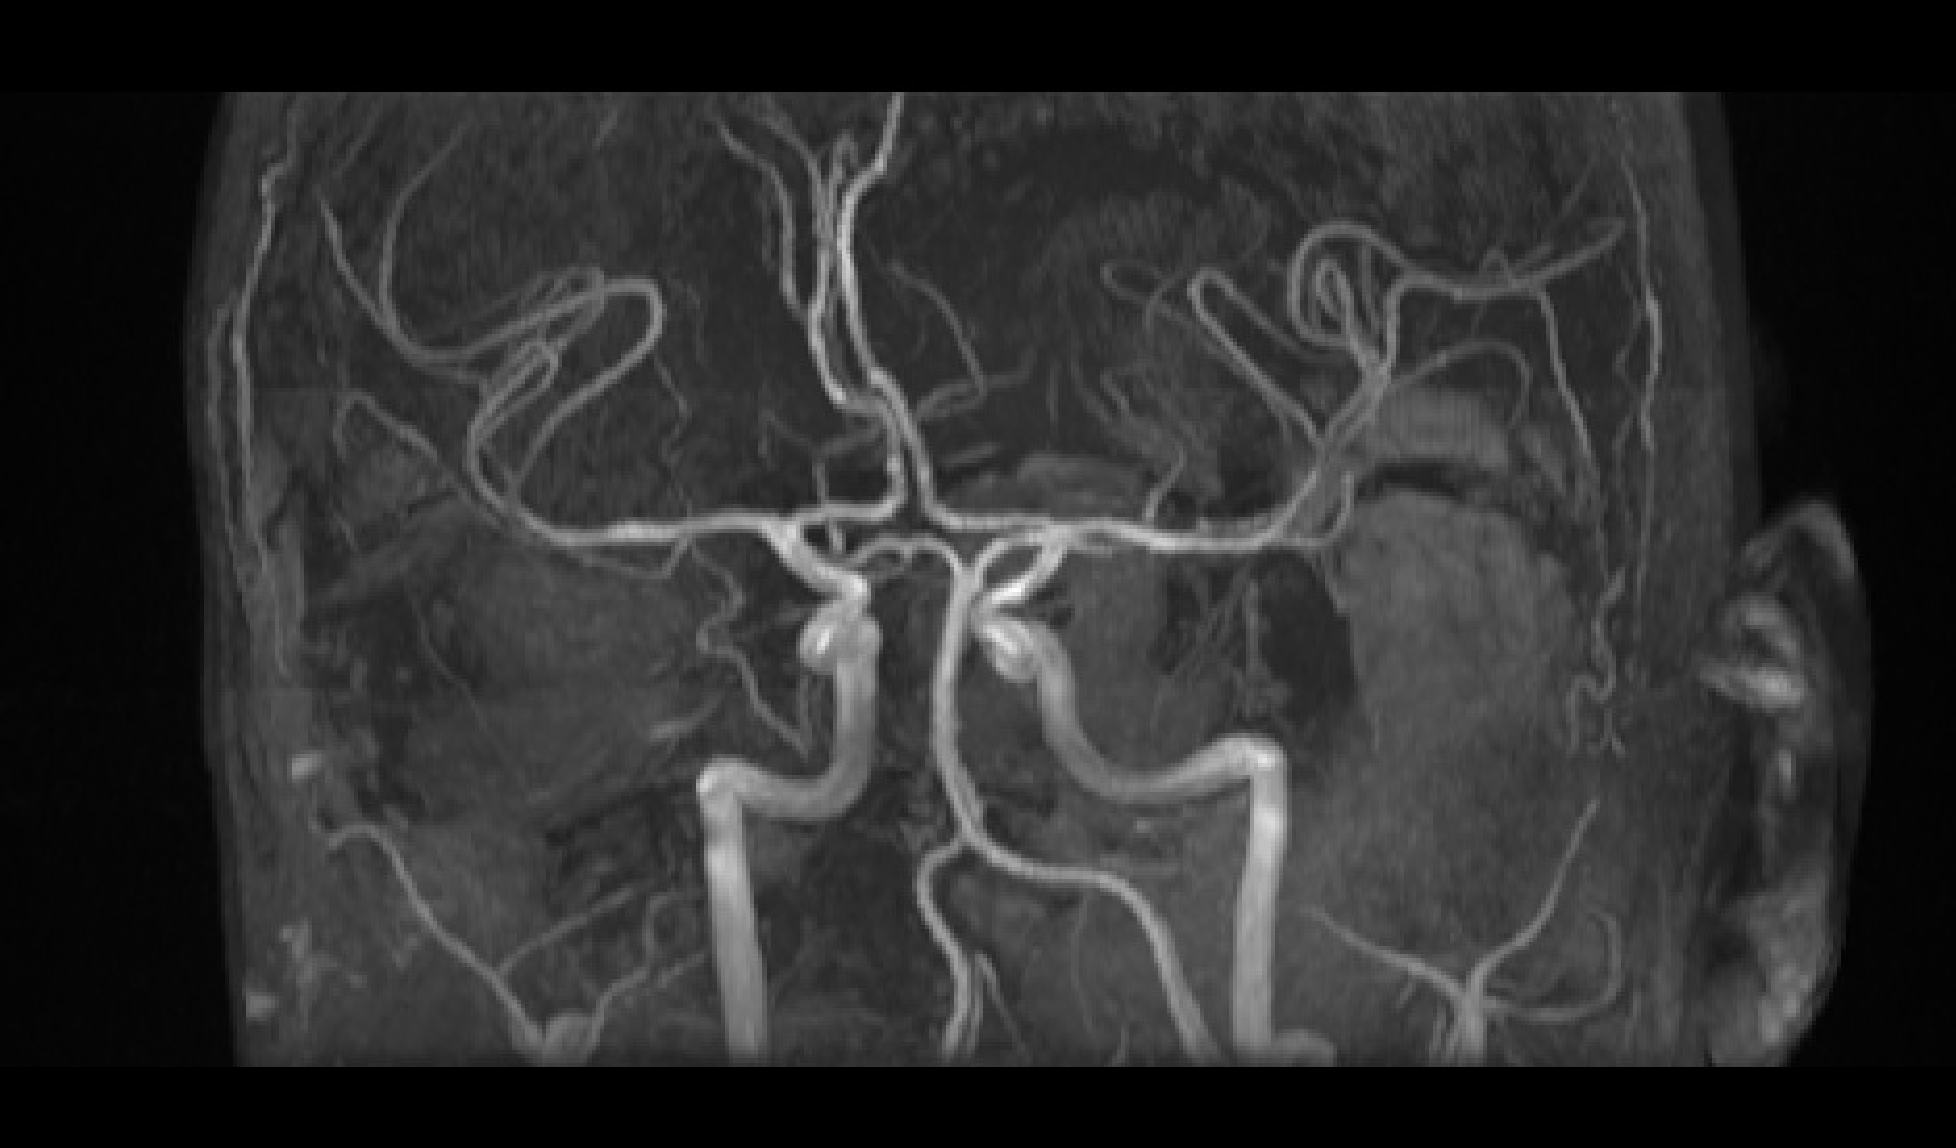
\includegraphics[width=\largefig]{chapters/kvs-2/pdf/kentus.pdf}
  \caption{An image of a patient-specific Circle of Willis (of the second author) obtained with magnetic resonance angiography.}
  \label{fig:kvs-2:circle_kent}
\end{figure}

Aneurysms are relatively common. As many as 1--6\% of the population
develop aneurysms during their
lifetime \citep{Weir2002}. Unfortunately, aneurysms often rupture at a
relatively early age. The average age of rupture is 52
years \citep{Humphrey2001}. An intracranial aneurysm is a dilatation
of the blood vessel wall, and the reasons for initialization, growth
and rupture of aneurysms are largely unknown.  What is known is that
increased wall shear stress (WSS) affects vascular endothelial cell
turnover \citep{DAVIESREMUZZIGORDONEtAl1986}, that aneurysms may grow
in the direction of low wall shear
stress \citep{BousselRayzMcCullochEtAl2008}, and that flow pattern and
impingement zones affect the possibility of
rupture \citep{CebralCastroBurgessEtAl2005}. The vessel wall clearly
responds to mechanical stimuli and this is the reason why wall shear
stress is believed to be of special importance when trying to
understand the pathogenesis of intracranial aneurysms. It is also
known that the cerebral arteries lack perivascular support and the
walls are relatively thin relative to the rest of the intracranial
vasculature \citep{Humphrey2001,Stehbens1975}.  Furthermore, the
anatomy of cerebral vessels varies greatly. Only around 50\% of the
general population have a complete and well-balanced circle; the rest
either have under-developed vessels or the vessels are missing
completely \citep{Fung1984}. Gender, ethnicity and lifestyle have
shown to be of
importance \citep{MhurchuAndersonJamrozikEtAl2001,LongstrethNelsonKoepsellEtAl1994,KongableLanzinoGermansonEtAl1996}.

%------------------------------------------------------------------------------
\section{Preliminaries}

\subsection{Stress calculation}

We noted above that wall shear stress is of importance in
computational hemodynamics. In Figure~\ref{fig:kvs-2:stress_code}, we
demonstrate how to compute stresses in FEniCS from a computed velocity
field~$u$ and pressure field~$p$. We start from the definition of the
stress tensor $\sigma(u,p) = 2 \nu \varepsilon (u) - p I$, where the
$\varepsilon(u) = \frac{1}{2}(\nabla u + \nabla u^{\top})$ is the symmetric
velocity gradient. Then, the normal and tangential components of the
stress are computed, where the tangential component is computed by
subtracting the normal component from the traction $T = \sigma \cdot
n$. Here, $n$ is the inward-pointing unit normal from the vessel
wall. In the code, \emp{n} is the outward-pointing unit normal. To
compute the shear and normal stresses as fields over the mesh, we test
the stresses against piecewise constant test functions scaled by the
inverse area of each facet. We thus obtain a piecewise constant
representation of the stress which on each cell is equal to the
average stress on that cell.

\begin{figure}
\bwfig
\begin{python}
# Compute stress tensor
sigma = 2*nu*epsilon(u) - p*Identity(len(u))

# Compute surface traction
n = FacetNormal(mesh)
T = -sigma*n

# Compute normal and tangential components
Tn = inner(T, n) # scalar-valued
Tt = T - Tn*n    # vector-valued

# Piecewise constant test functions
scalar = FunctionSpace(mesh, "DG", 0)
vector = VectorFunctionSpace(mesh, "DG", 0)
v = TestFunction(scalar)
w = TestFunction(vector)

# Assemble piecewise constant functions for stress
normal_stress = Function(scalar)
shear_stress = Function(vector)
Ln = (1 / FacetArea(mesh))*v*Tn*ds
Lt = (1 / FacetArea(mesh))*inner(w, Tt)*ds
assemble(Ln, tensor=normal_stress.vector())
assemble(Lt, tensor=shear_stress.vector())
\end{python}
  \caption{Computing normal and shear stresses from computed
    velocity and pressure fields \emp{u} and \emp{p}.}
\label{fig:kvs-2:stress_code}\end{figure}

\subsection{Boundary conditions} \label{resistance_bcs}

For transient inlet boundary conditions, one option is to apply
velocity waveform data in the ICA from \citet{FordAlperinLeeEtAl2005},
where the average velocity was measured for seventeen young patients
at rest. The nondimensionalized velocity is illustrated in
Figure~\ref{fig:kvs-2:ford}. The inlet velocity profile is easy to
measure through the ICA or the VA using transcranial Doppler. This
enables patient-specific velocity measurements such as in the Circle of Willis
study in Section~\ref{cok}.

\begin{figure}
\bwfig
  \centering
  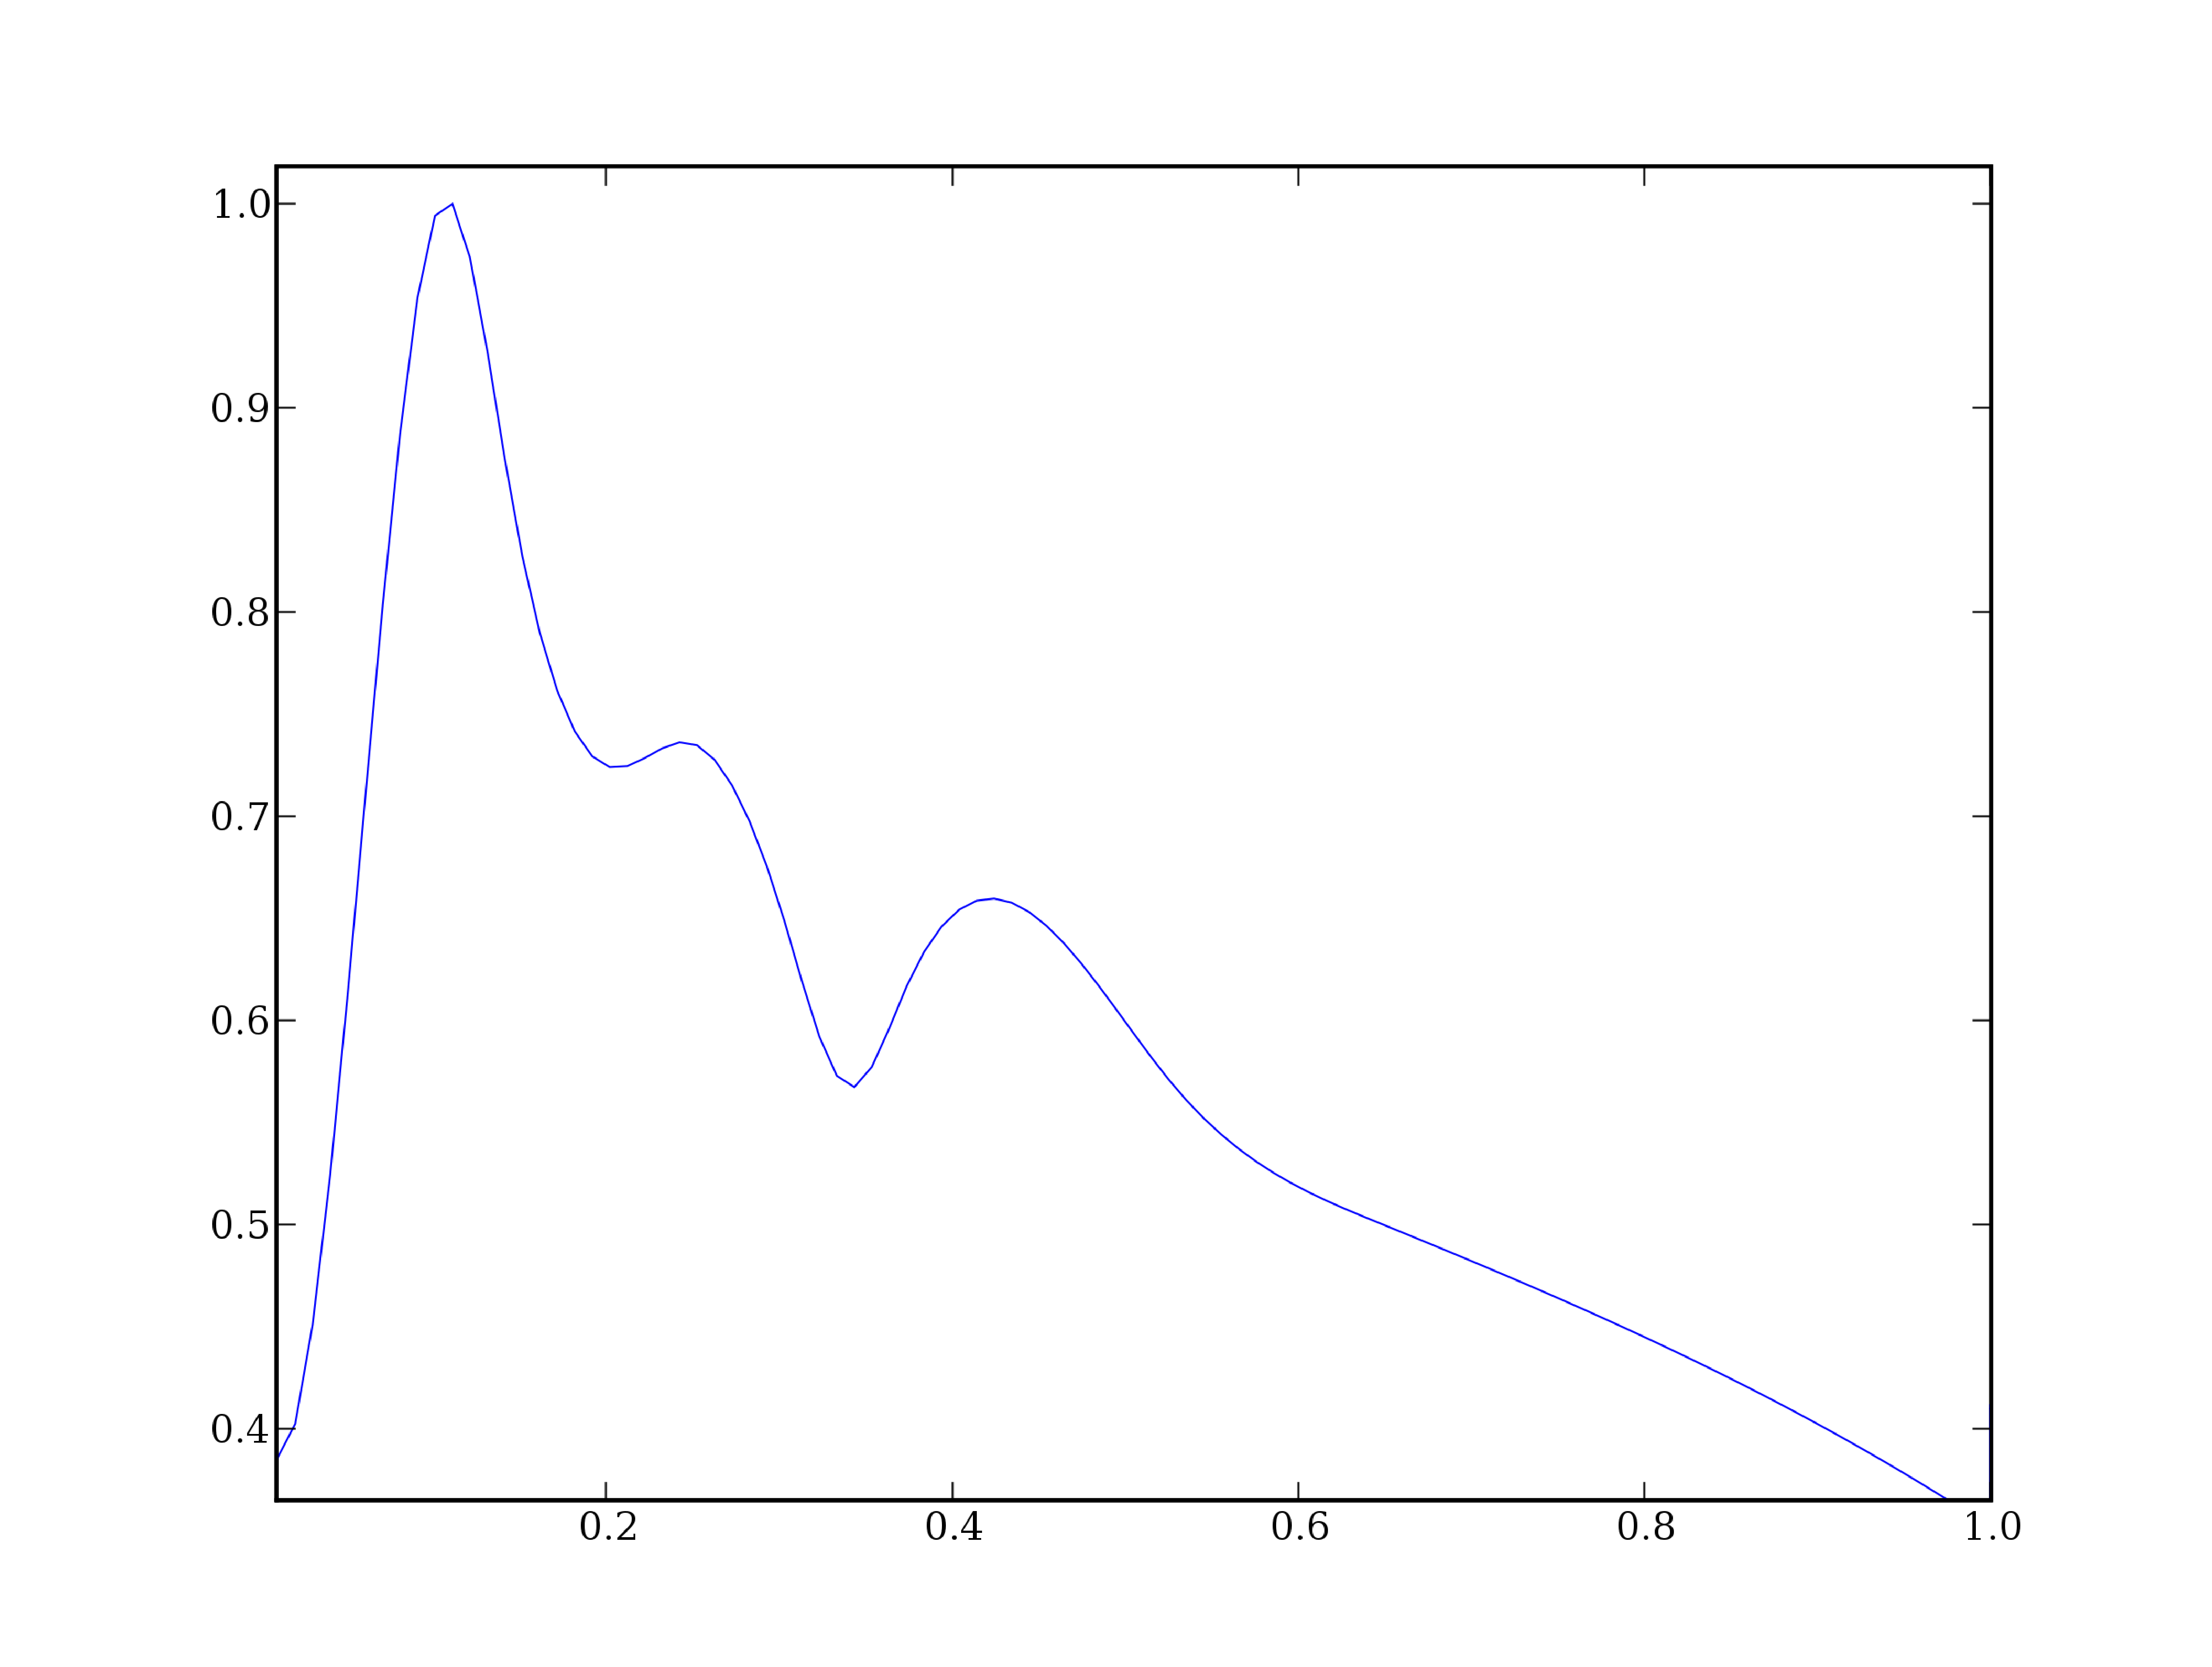
\includegraphics[width=\largefig]{chapters/kvs-2/pdf/systolic.pdf}
   \caption{Nondimensionalized ICA inlet velocity profile.}
\label{fig:kvs-2:ford}
\end{figure}

Further into the brain, the flow is divided into branches several
times, which makes the outflow difficult to measure, both because of
the thickness of the cranium and the decreasing size of the vessels.
The effect of outflow boundary conditions in a complex network of
blood vessels, such as in the Circle of Willis, is important to the
flow division and wall shear stress.

The simplest way to describe the outflow is by applying a zero
traction boundary condition at the outflow. However, the flow division
in a bifurcation is dependent on the downstream vasculature, and the
zero traction boundary condition does not capture this very
well. Therefore, to model the peripheral resistance, a resistance
model may be used for the pressure, while a Neumann condition
(${\partial u / \partial n} = 0 $) is applied to the velocity. The
value of the resistance boundary condition is proportional to the
flow; that is, the pressure at the outlet~$\Gamma$ is modeled as,
\begin{equation} \label{kvs-2:eq:resistancebc}
  p = p_0 + R = p_0 + C \int_\Gamma u \cdot n \ds,
\end{equation}
where the resistance coefficient~$C$ was set according to
Table~\ref{resistance_coeff}, $p_0$ is the mean intracranial arterial
pressure (85 mmHg), which is applied to the inlet, and $u$ is the
velocity. The coefficients in Table~\ref{resistance_coeff} are
from \citet{AlastrueyParkerPeiroEtAl2007} and show a clear relation
between the diameter of the vessel and the resistance coefficient. The
implementation of the resistance boundary condition is shown in
Figure~\ref{fig:kvs-2:resistance_code}.

\begin{table}
  \centering
  \begin{tabular}{l*{7}{r}r}
    \toprule
    Artery & $C$ $ [10^9 \mathrm{Pa} \cdot \mathrm{s}  \cdot \mathrm{m}^{-3}]$ & Radius [mm]\\
    \midrule
    Thoracic Aorta			&  0.18 &  	9.99\\
    External Carotid Artery  	& 5.43   &	1.50\\
    Middle Cerebral Artery  	& 5.97   &	1.43\\
    Anterior Communicating Artery  	& 8.48   &	1.20\\
    Posterior Communicating Artery  & 11.08   &	1.05\\
    \bottomrule
  \end{tabular}
  \caption{Resistance boundary condition coefficient, $C$,
    for selected arteries of varying size; see Equation~\eqref{kvs-2:eq:resistancebc}.}
  \label{resistance_coeff}
\end{table}

\begin{figure}
\bwfig
\begin{python}
# Outflow boundary value for pressure
def OutflowBoundaryValue(self, i):
    u = self.problem.u
    n = FacetNormal(self.problem.mesh)
    flux = dot(u, n)*ds(i)
    Q = assemble(flux,
                 exterior_facet_domains=\
                 self.problem.sub_domains)
    C = 5.97*10**(-3)
    p0 = 11332.0*10**(-6) # 85 mmHg to Pascal
    R = (C*Q + p0)*(rhoinv)
    return R
\end{python}
\caption{Calculation of the outflow boundary value for the pressure. The
numbers have been multiplied with $10^{-3}$
and $10^{-6}$ to convert from SI units to millimeters, milliseconds
and grams.}
\label{fig:kvs-2:resistance_code}
\end{figure}

The effect of the resistance boundary condition may bee seen in
Figure~\ref{fig:kvs-2:resistance_bcs_fig} where the mass flux over two
outlets in the canine geometry in Section~\ref{dog_study} is
calculated using both zero traction and a resistance boundary
condition. The resulting flow division is clearly more evenly
distributed (colored in red) between the daughter vessels, which
intuitively also makes sense since the vessels reconnect further
downstream. The method requires an iteration over a few cardiac cycles
in order to converge.

\begin{figure}
\bwfig
  \centering
  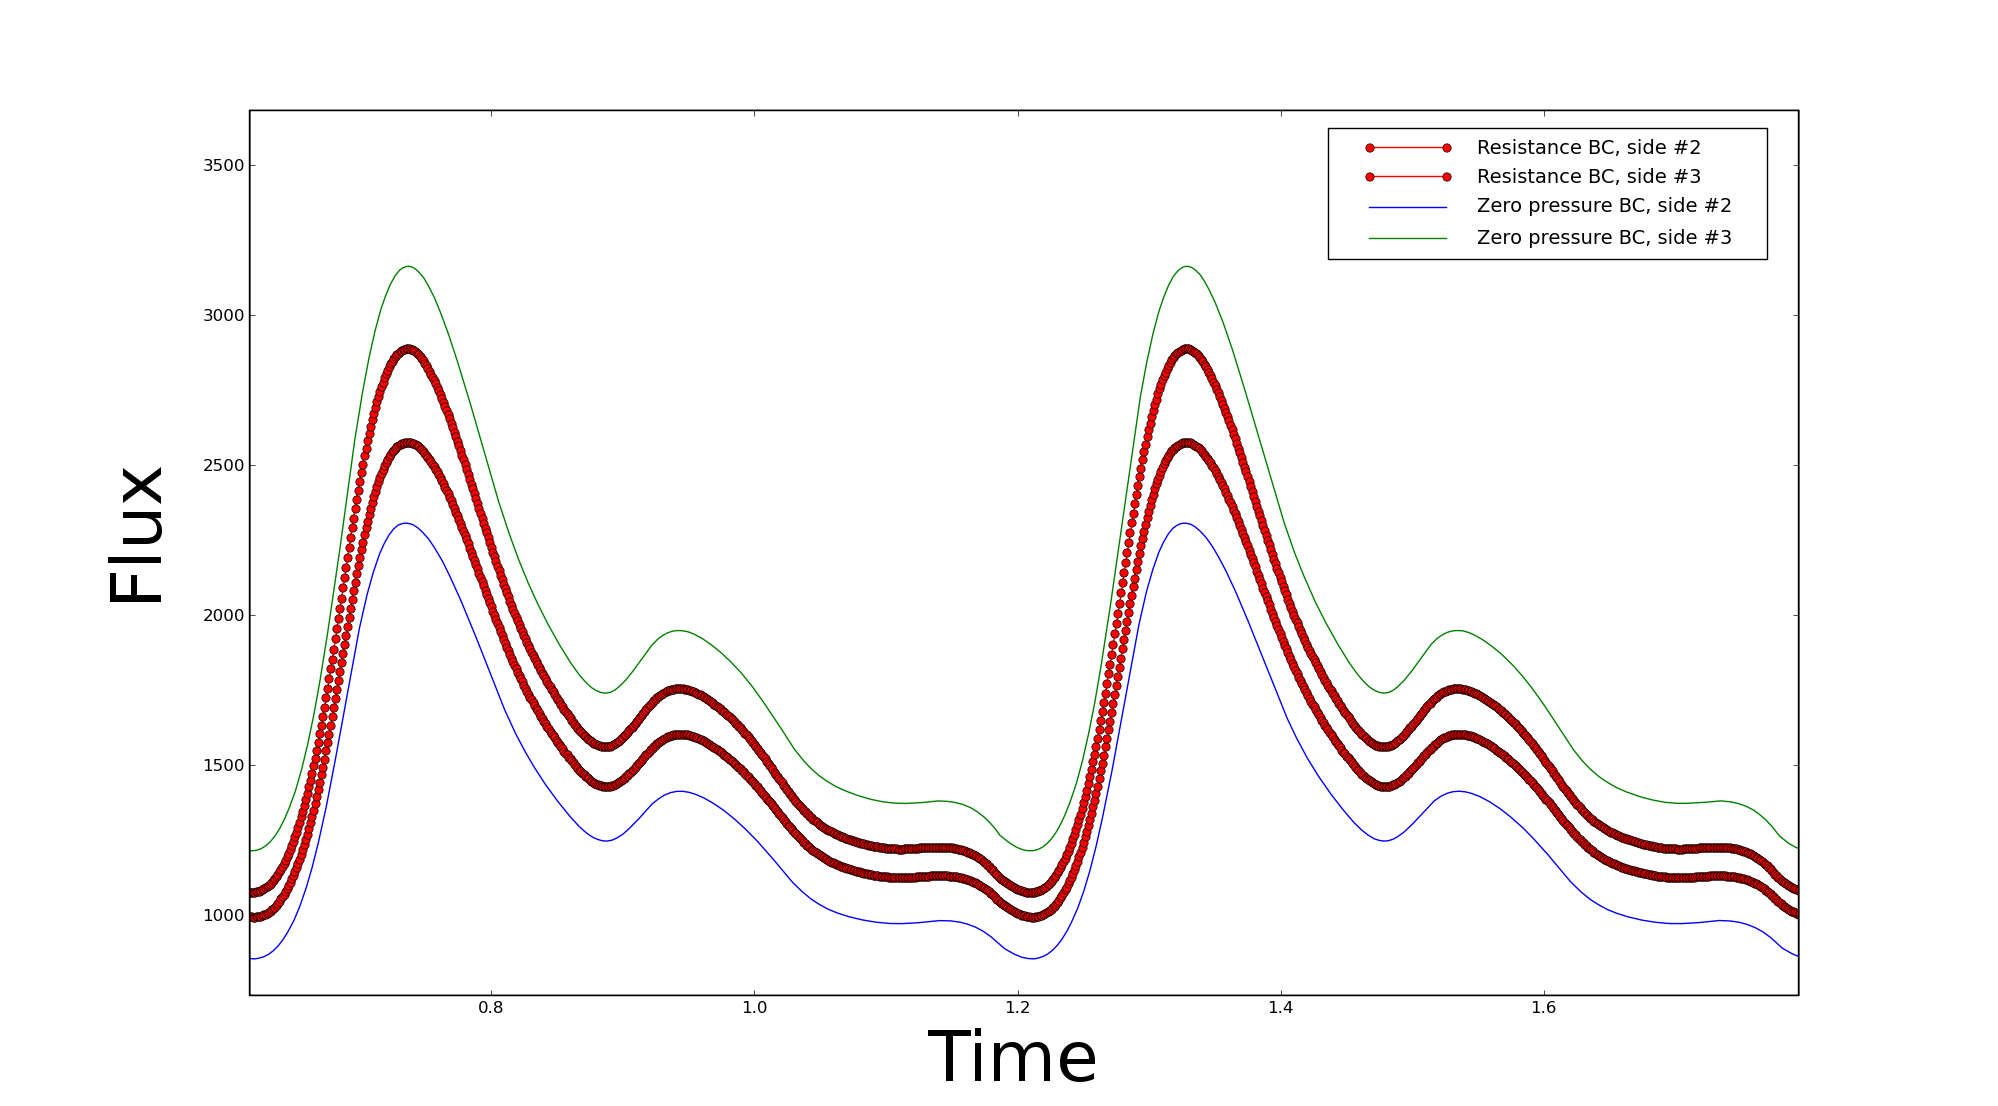
\includegraphics[width=\largefig]{chapters/kvs-2/png/zero_dp_vs_res.png}
  \caption{Figure showing the difference of outflow
    flux when a resistance boundary condition (as described in section
    ~\ref{resistance_bcs}) is applied versus zero traction. When a
    resistance boundary condition is used, the flow is more evenly
    distributed between the two vessel outlets (red curves), compared
    to the case when a zero traction condition is used (blue and green
    curves).}
  \label{fig:kvs-2:resistance_bcs_fig}
\end{figure}

\subsection{Anatomical modeling} \label{vmtk}

\begin{figure}
\bwfig
  \ffigbox{\caption{Image segmentation process; from MRI to
      mesh.}\label{fig:kvs-2:imagseg}}
          {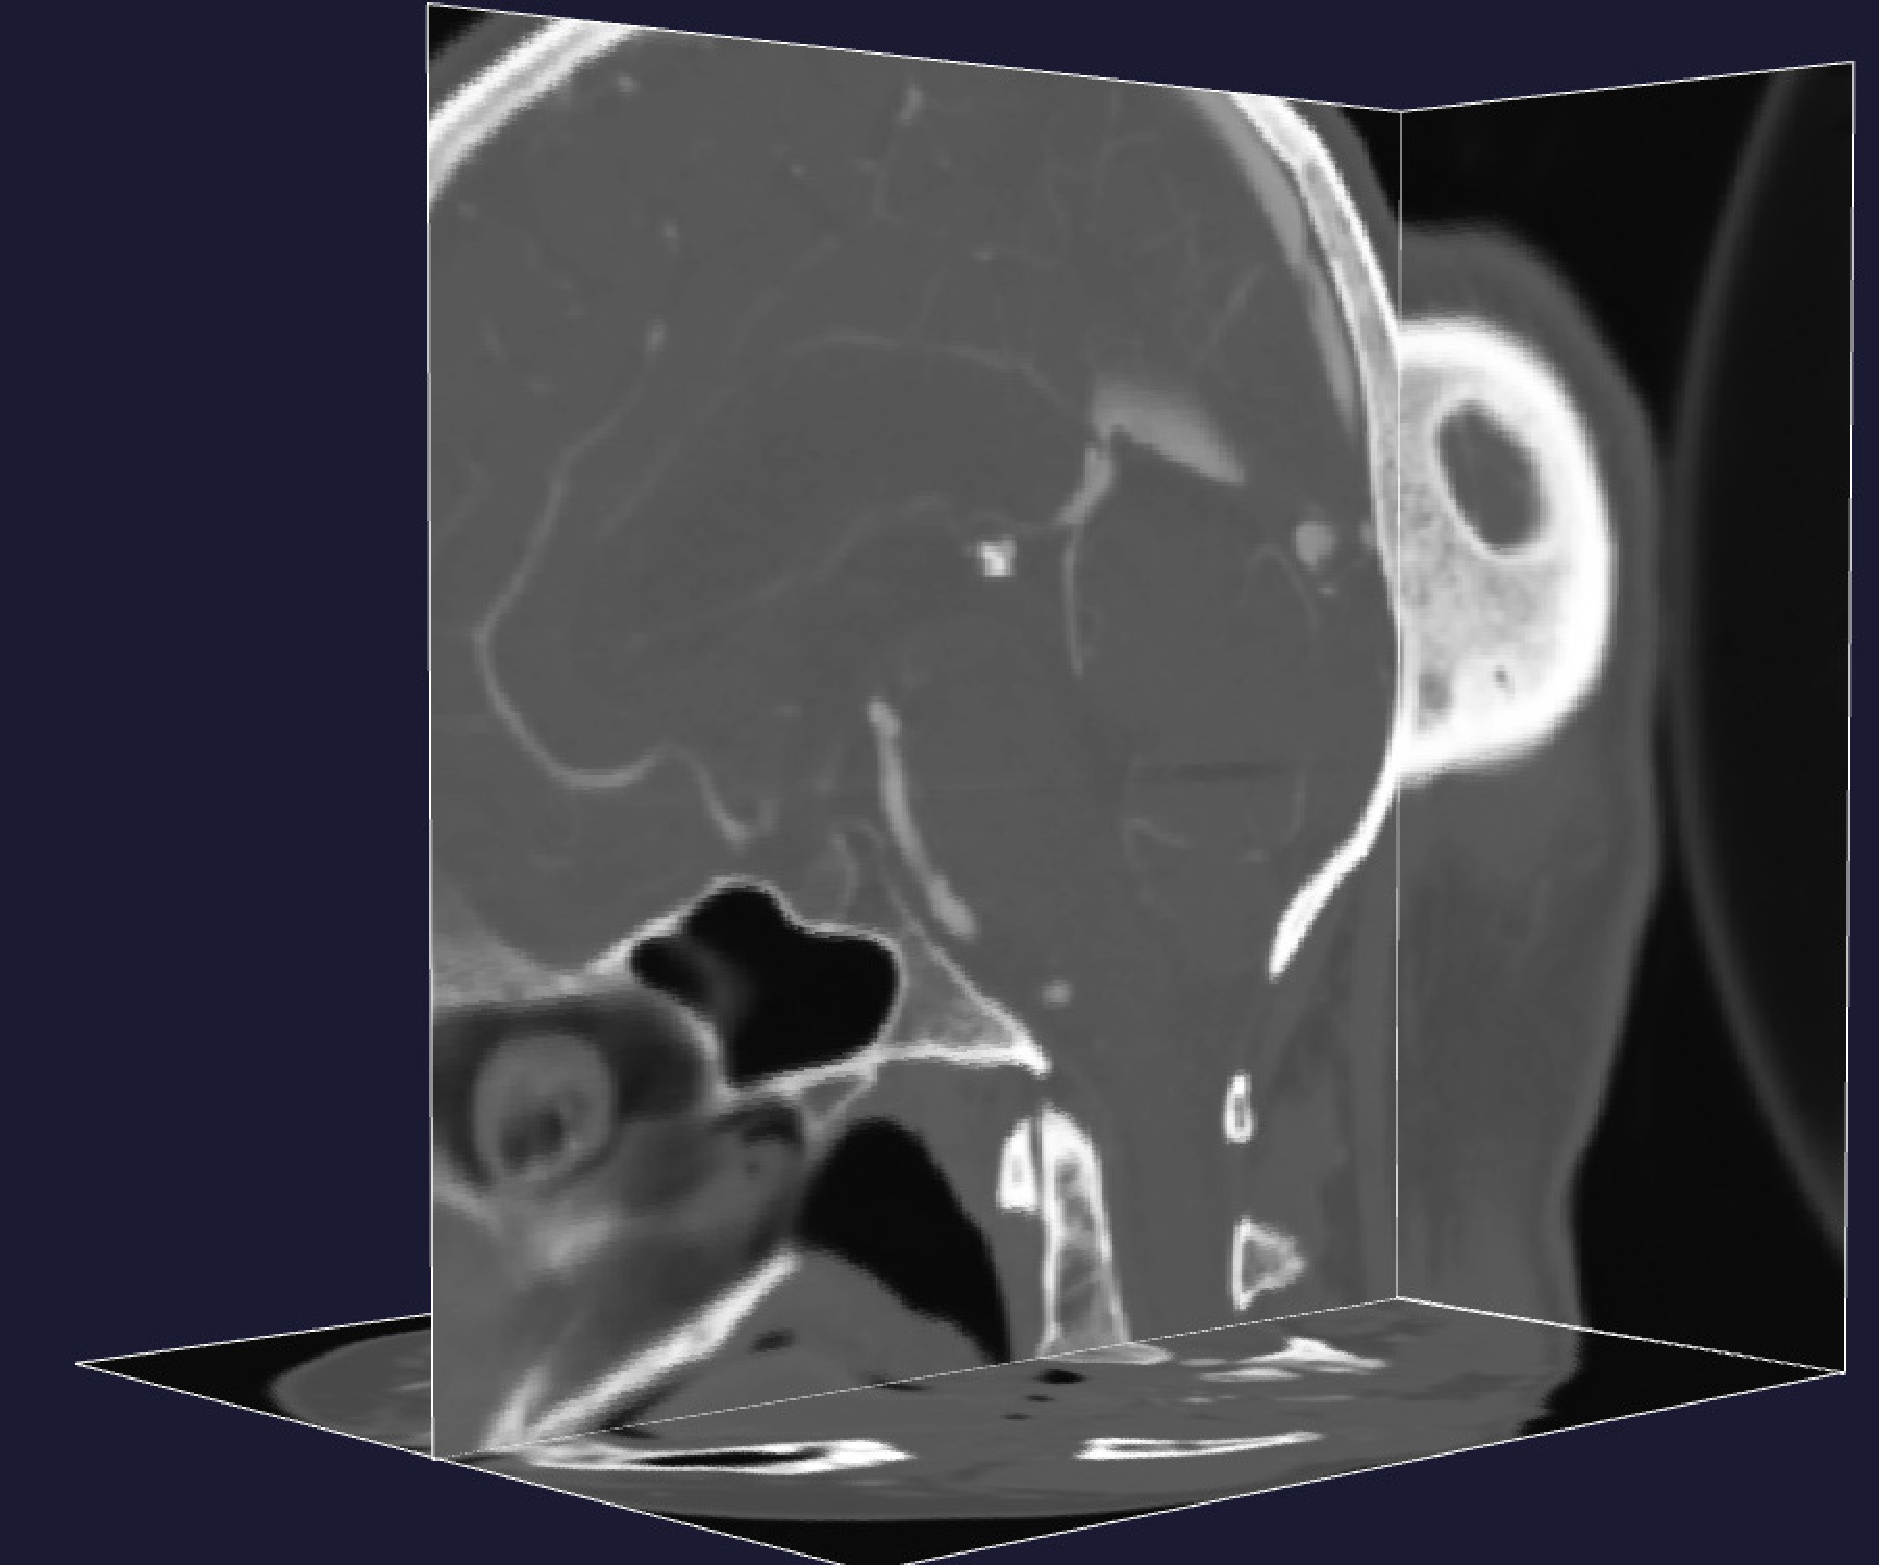
\includegraphics[width=\threefigsfull]{chapters/kvs-2/pdf/stacks.pdf}
            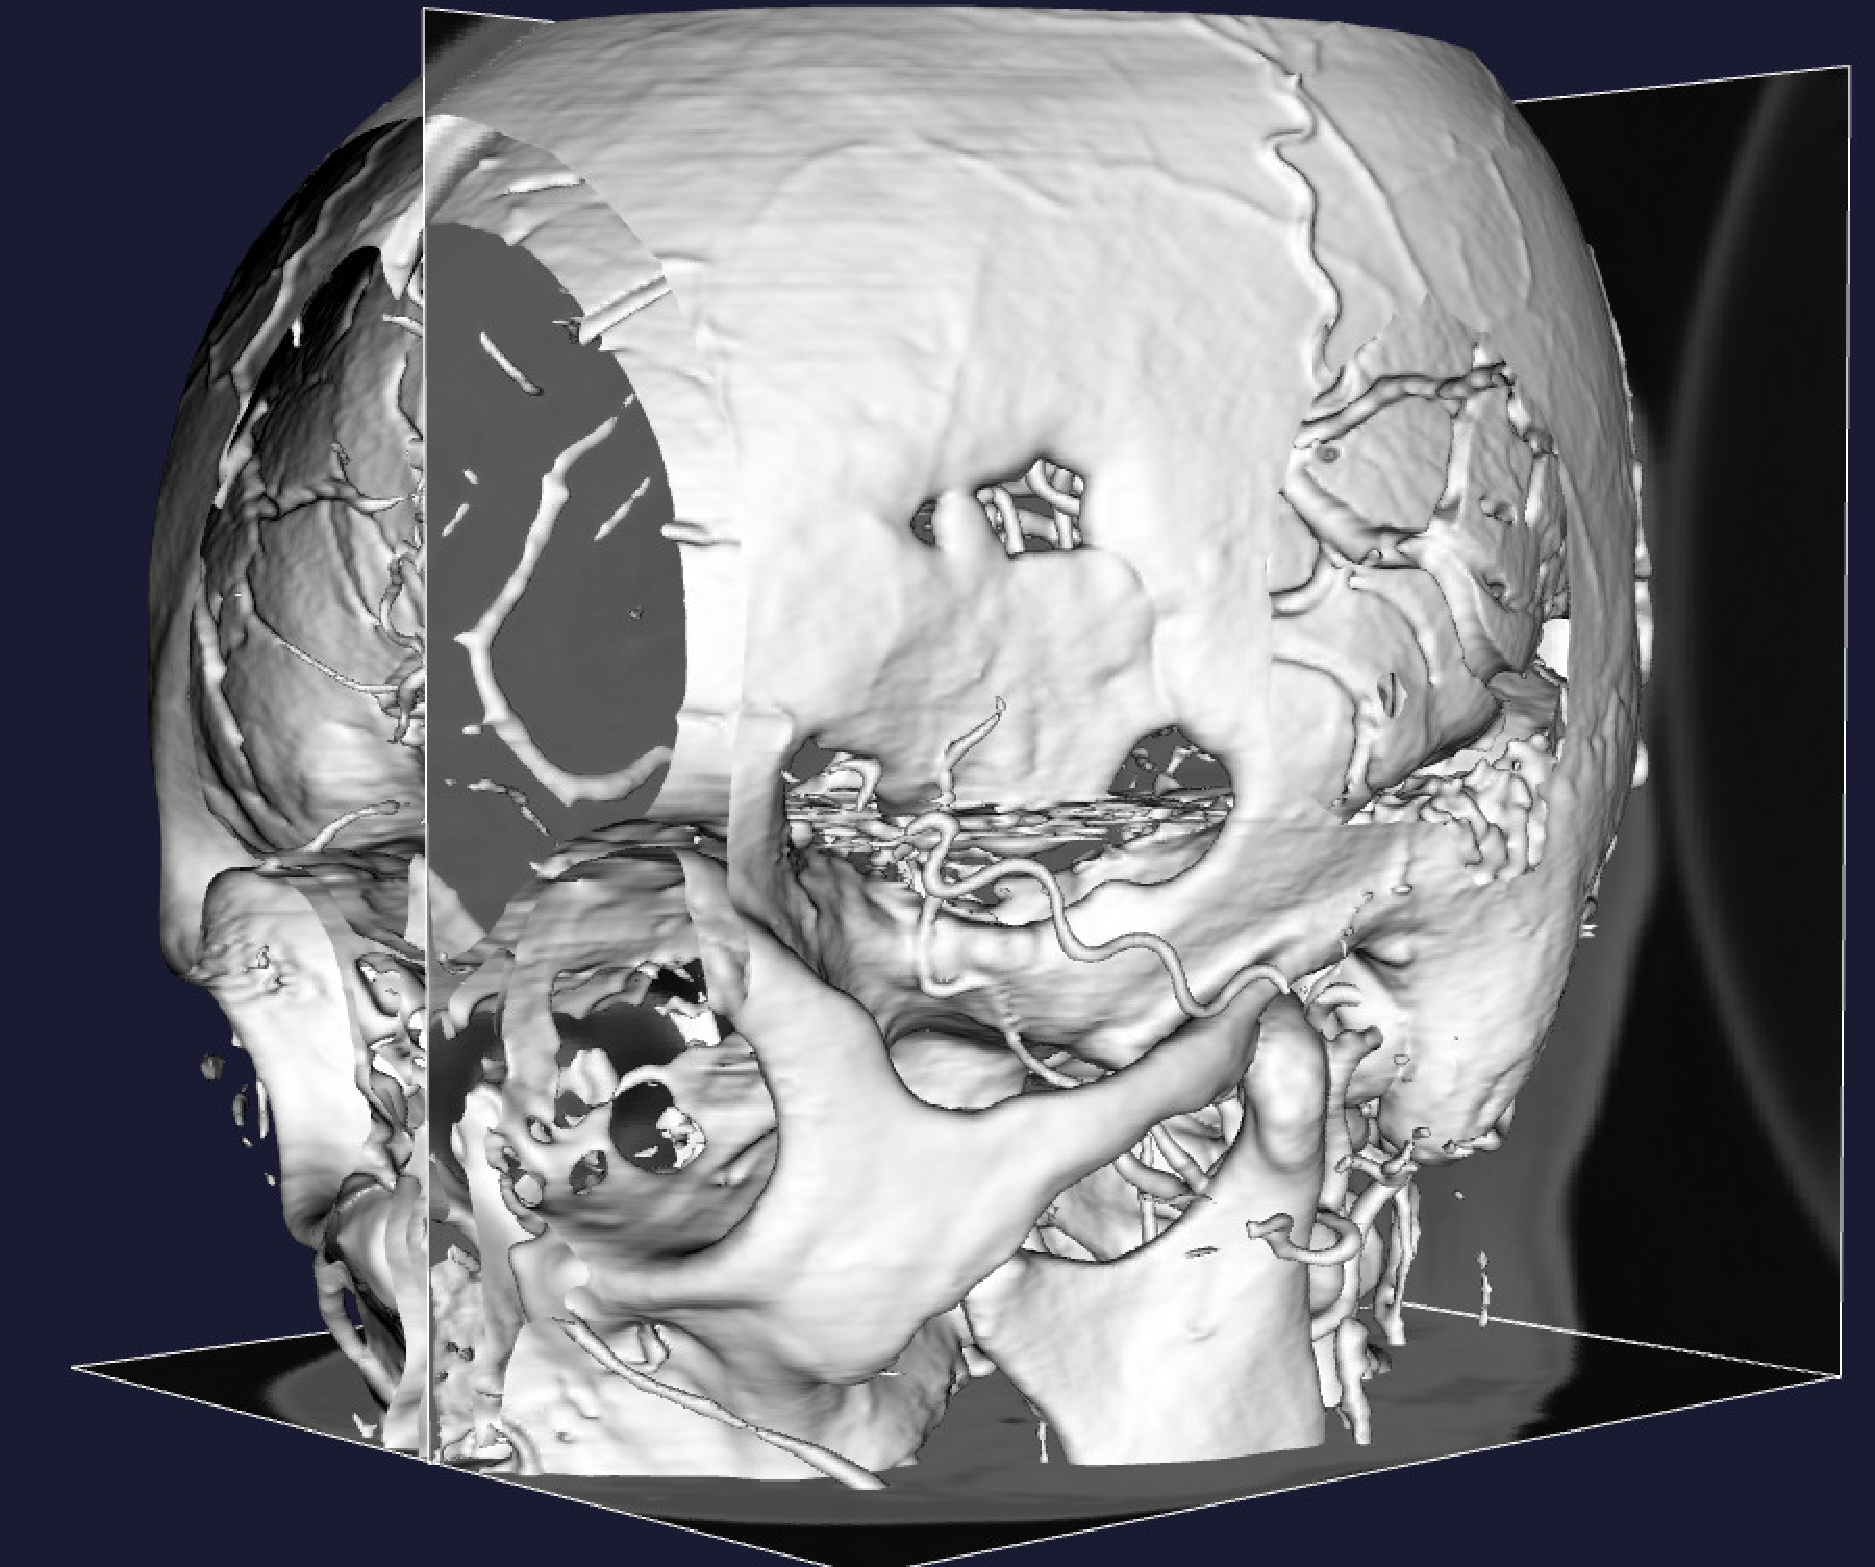
\includegraphics[width=\threefigsfull]{chapters/kvs-2/pdf/3d.pdf}
            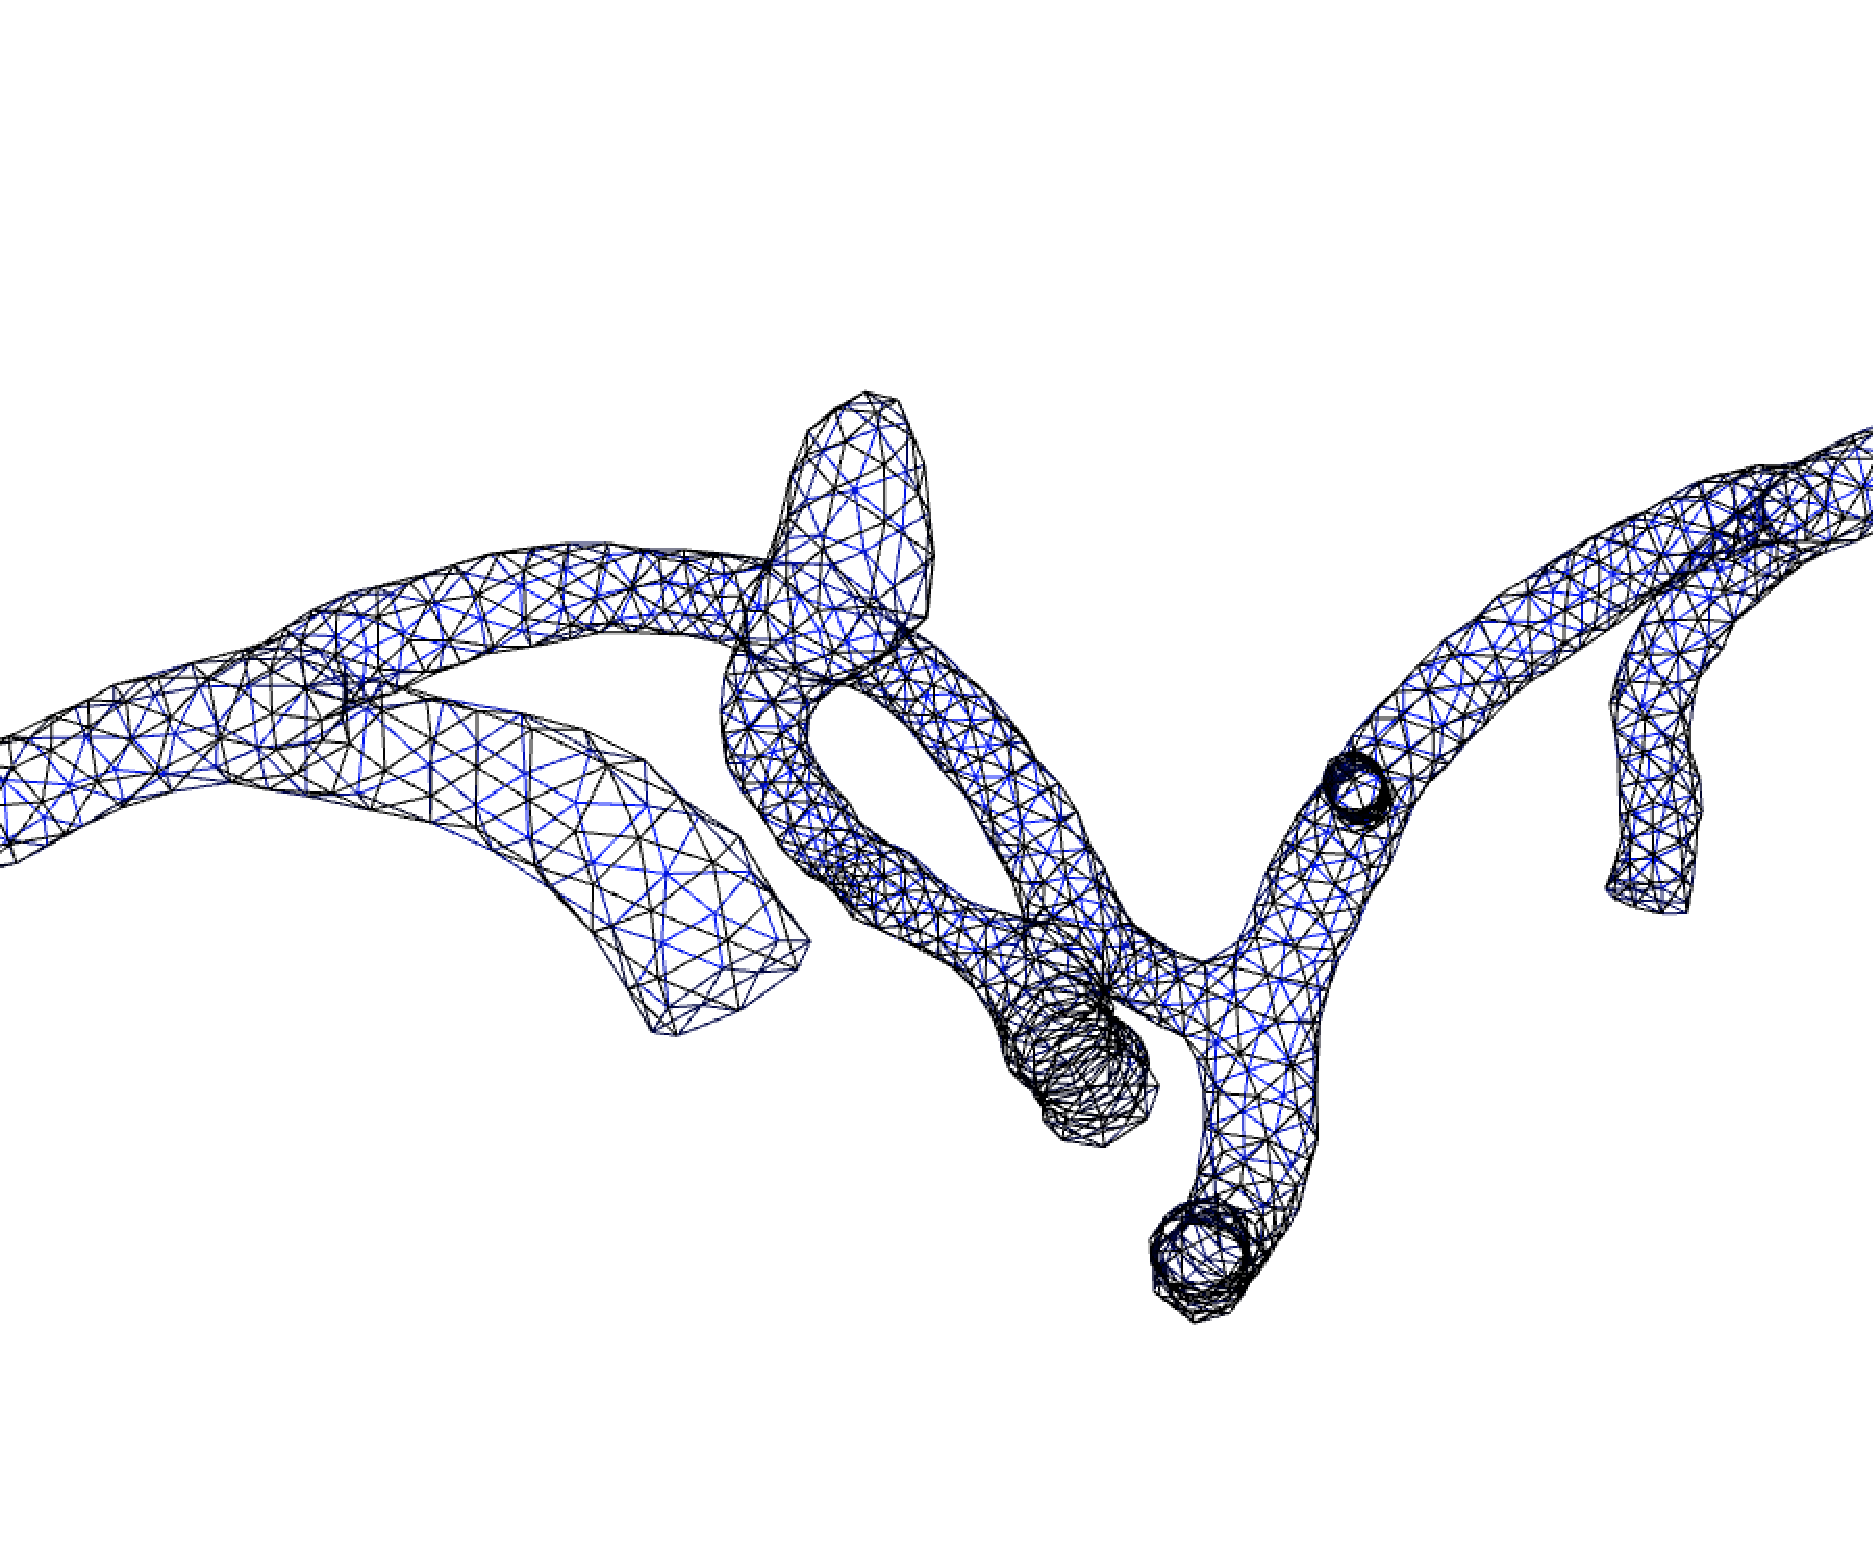
\includegraphics[width=\threefigsfull]{chapters/kvs-2/pdf/viper3.pdf}}
\end{figure}

Patient-specific geometries are obtained from Computed Tomography
Angiography (CTA) or Magnetic Resonance Angiography (MRA) images as
follows. A stack of 2D images is used as input to the \citet{vmtk} (VMTK),
where a 3D surface model is generated based upon the light intensity
in the pictures using level set techniques. A volume is then created
from the surface, from which a mesh can be generated. This process is
illustrated in Figure~\ref{fig:kvs-2:imagseg}, where the mesh of a
blood vessel extracted from the geometry is shown to the right. This
mesh is used as input to the flow solver.

%------------------------------------------------------------------------------
\section{Gender differences in the intracranial vasculature} \label{gender}

In this section, we present an overview of a recent study
by \citet{LindekleivValen-SendstadMorganEtAl2010} where it is shown
that on average, women have larger shear stresses than men in two
intracranial bifurcations.

\subsection{Background}

Females are more likely to harbor intracranial aneurysms than men and,
consequently, more frequently develop subarachnoid hemorrhage
(SAH) \citep{EdenMeurerSanchezEtAl2008}. The reason is not known, but
studies suggest an increased risk of aneurysm rupture after the age of
fifty, in the postmenopausal years. This might indicate the influence
of hormonal factors on the vessel wall. This hypothesis is supported
by the reduced risk of SAH with increasing number of
births given by the female. However, studies
have failed to prove a decisive correlation between hormonal factors
and the risk of SAH. Another hypothesis is that high values of wall
shear stress may influence the initialization of aneurysms. With
measurements of radii and angles of intracranial bifurcations
available from a previous study in our group,
see \citet{IngebrigtsenMorganFaulderEtAl2004}, we therefore wished to
reanalyze the data and calculate the gender specific hemodynamic
forces by numerical simulations.

\subsection{Method}

Measurements of 49 patients were performed to obtain the geometric
quantities of the MCA and ICA bifurcations. The averaged values for
the diameters were used to create one idealized bifurcation of the MCA
and ICA for both females and males. The model basically consists of
three cylinders connected with a smoothing at the interface to give a
physiologically plausible appearance.

Average gender specific blood flow velocity measurements from the ICA
and MCA from \citet{KrejzaSzydlikLiebeskindEtAl2005} were used as
inflow boundary conditions in the simulations. Table~\ref{bcs}
summarizes the input values to the simulations.
At the outflows,
we have applied a resistance boundary condition as described in
Section~\ref{resistance_bcs}.

\subsection{Results}

Table~\ref{bcs} shows that there is a significant gender difference in
the diameters for the MCA. For the ICA, there are only statistically
significant sex differences in the vessel size of the parent vessel
and the smallest branch. CFD simulations show both increased wall
shear stress and a larger affected area in the female MCA
(Figure~\ref{fig:kvs-2:mca_wss_res}) and ICA
(Figure~\ref{fig:kvs-2:ica_wss_res}) bifurcations. The maximum wall
shear stress in the MCA bifurcations was 33.17~Pa for females and
27.82~Pa for males. Similar results for ICA were 15.20~Pa for females
and~10.10~Pa for males. The values are reflected by a higher pressure
drop in the female than in the male bifurcations (664 vs. 502~Pa for MCA
and 344 vs. 202 Pa for ICA). For further discussion,
see \citet{LindekleivValen-SendstadMorganEtAl2010}.

\subsection{Discussion}

The above results are as expected from fluid mechanical reasoning,
except for the peak values in the vicinity of the bifurcations. Even
though the model is simple, the aim was to demonstrate a principle
with a potentially important application; that is, that WSS may be of
importance in the initialization and rupture of intracranial
aneurysms. Furthermore, the results correlate well with the fact that
women develop more aneurysms than men.

\begin{figure}
\bwfig
  \centering
  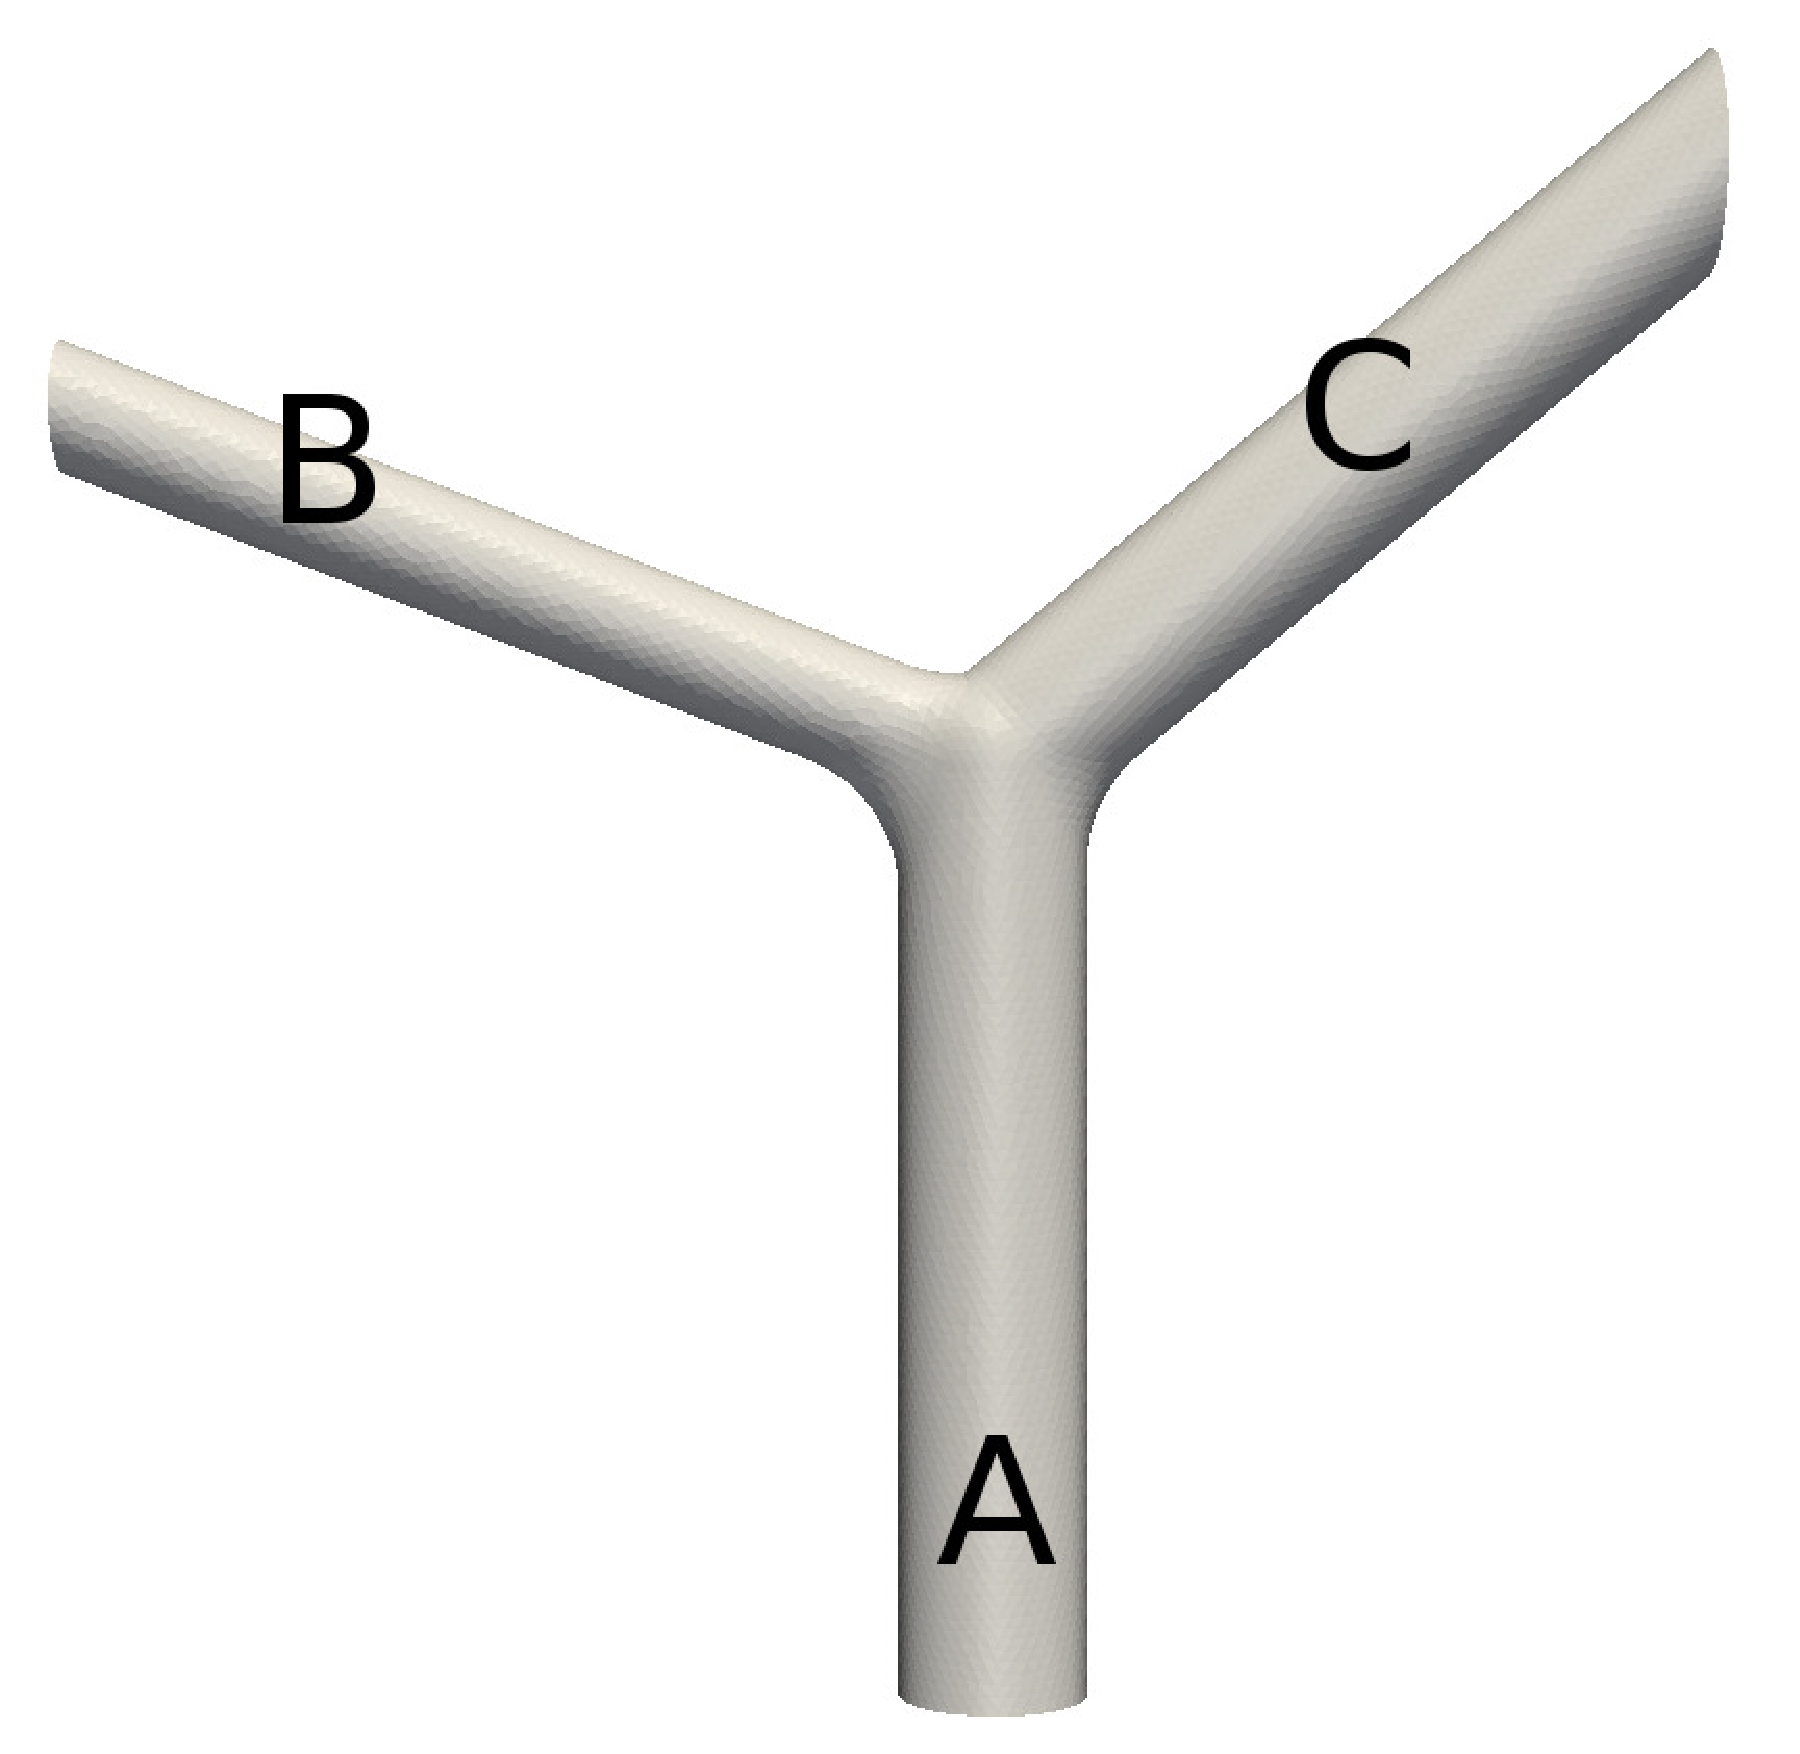
\includegraphics[width=\largefig]{chapters/kvs-2/pdf/bifurcation_clean.pdf}
  \caption{Idealized model of a bifurcation.}
  \label{fig:kvs-2:bif}
\end{figure}

\begin{table}
  \centering
  \begin{tabular}{l*{6}{c}r}
    \toprule
    & Male MCA & Female MCA & Male ICA & Female ICA \\
    \midrule
    $\alpha$	  & $49.7^\circ$ & $50.5^\circ$   & $62.8^\circ$ & $57.2^\circ$\\
    $\beta$		  & $68.8^\circ$ & $72.5^\circ$   & $49.7^\circ$ & $50.5^\circ$\\
    $A$~[mm]		  & 2.63 & 2.42   & 3.86 & 3.45\\
    $B$~[mm]           & 2.44 & 2.04   & 2.71 & 2.49\\
    $C$~[mm] 	  & 1.74 & 1.56   & 2.13 & 1.85\\
    $V$~[m/s]	  & 0.68   & 0.74     & 0.34   & 0.42  \\
    \bottomrule
  \end{tabular}
  \caption{Summary of angles, diameters and velocities for the
    bifurcation of Figure~\ref{fig:kvs-2:bif}, used in the
    simulations. The parameters $\alpha$ and $\beta$ are the angles
    between the prolongation of the parent artery and the vessels C
    and B, respectively.}
  \label{bcs}
\end{table}

\begin{figure}
\bwfig
  \centering
  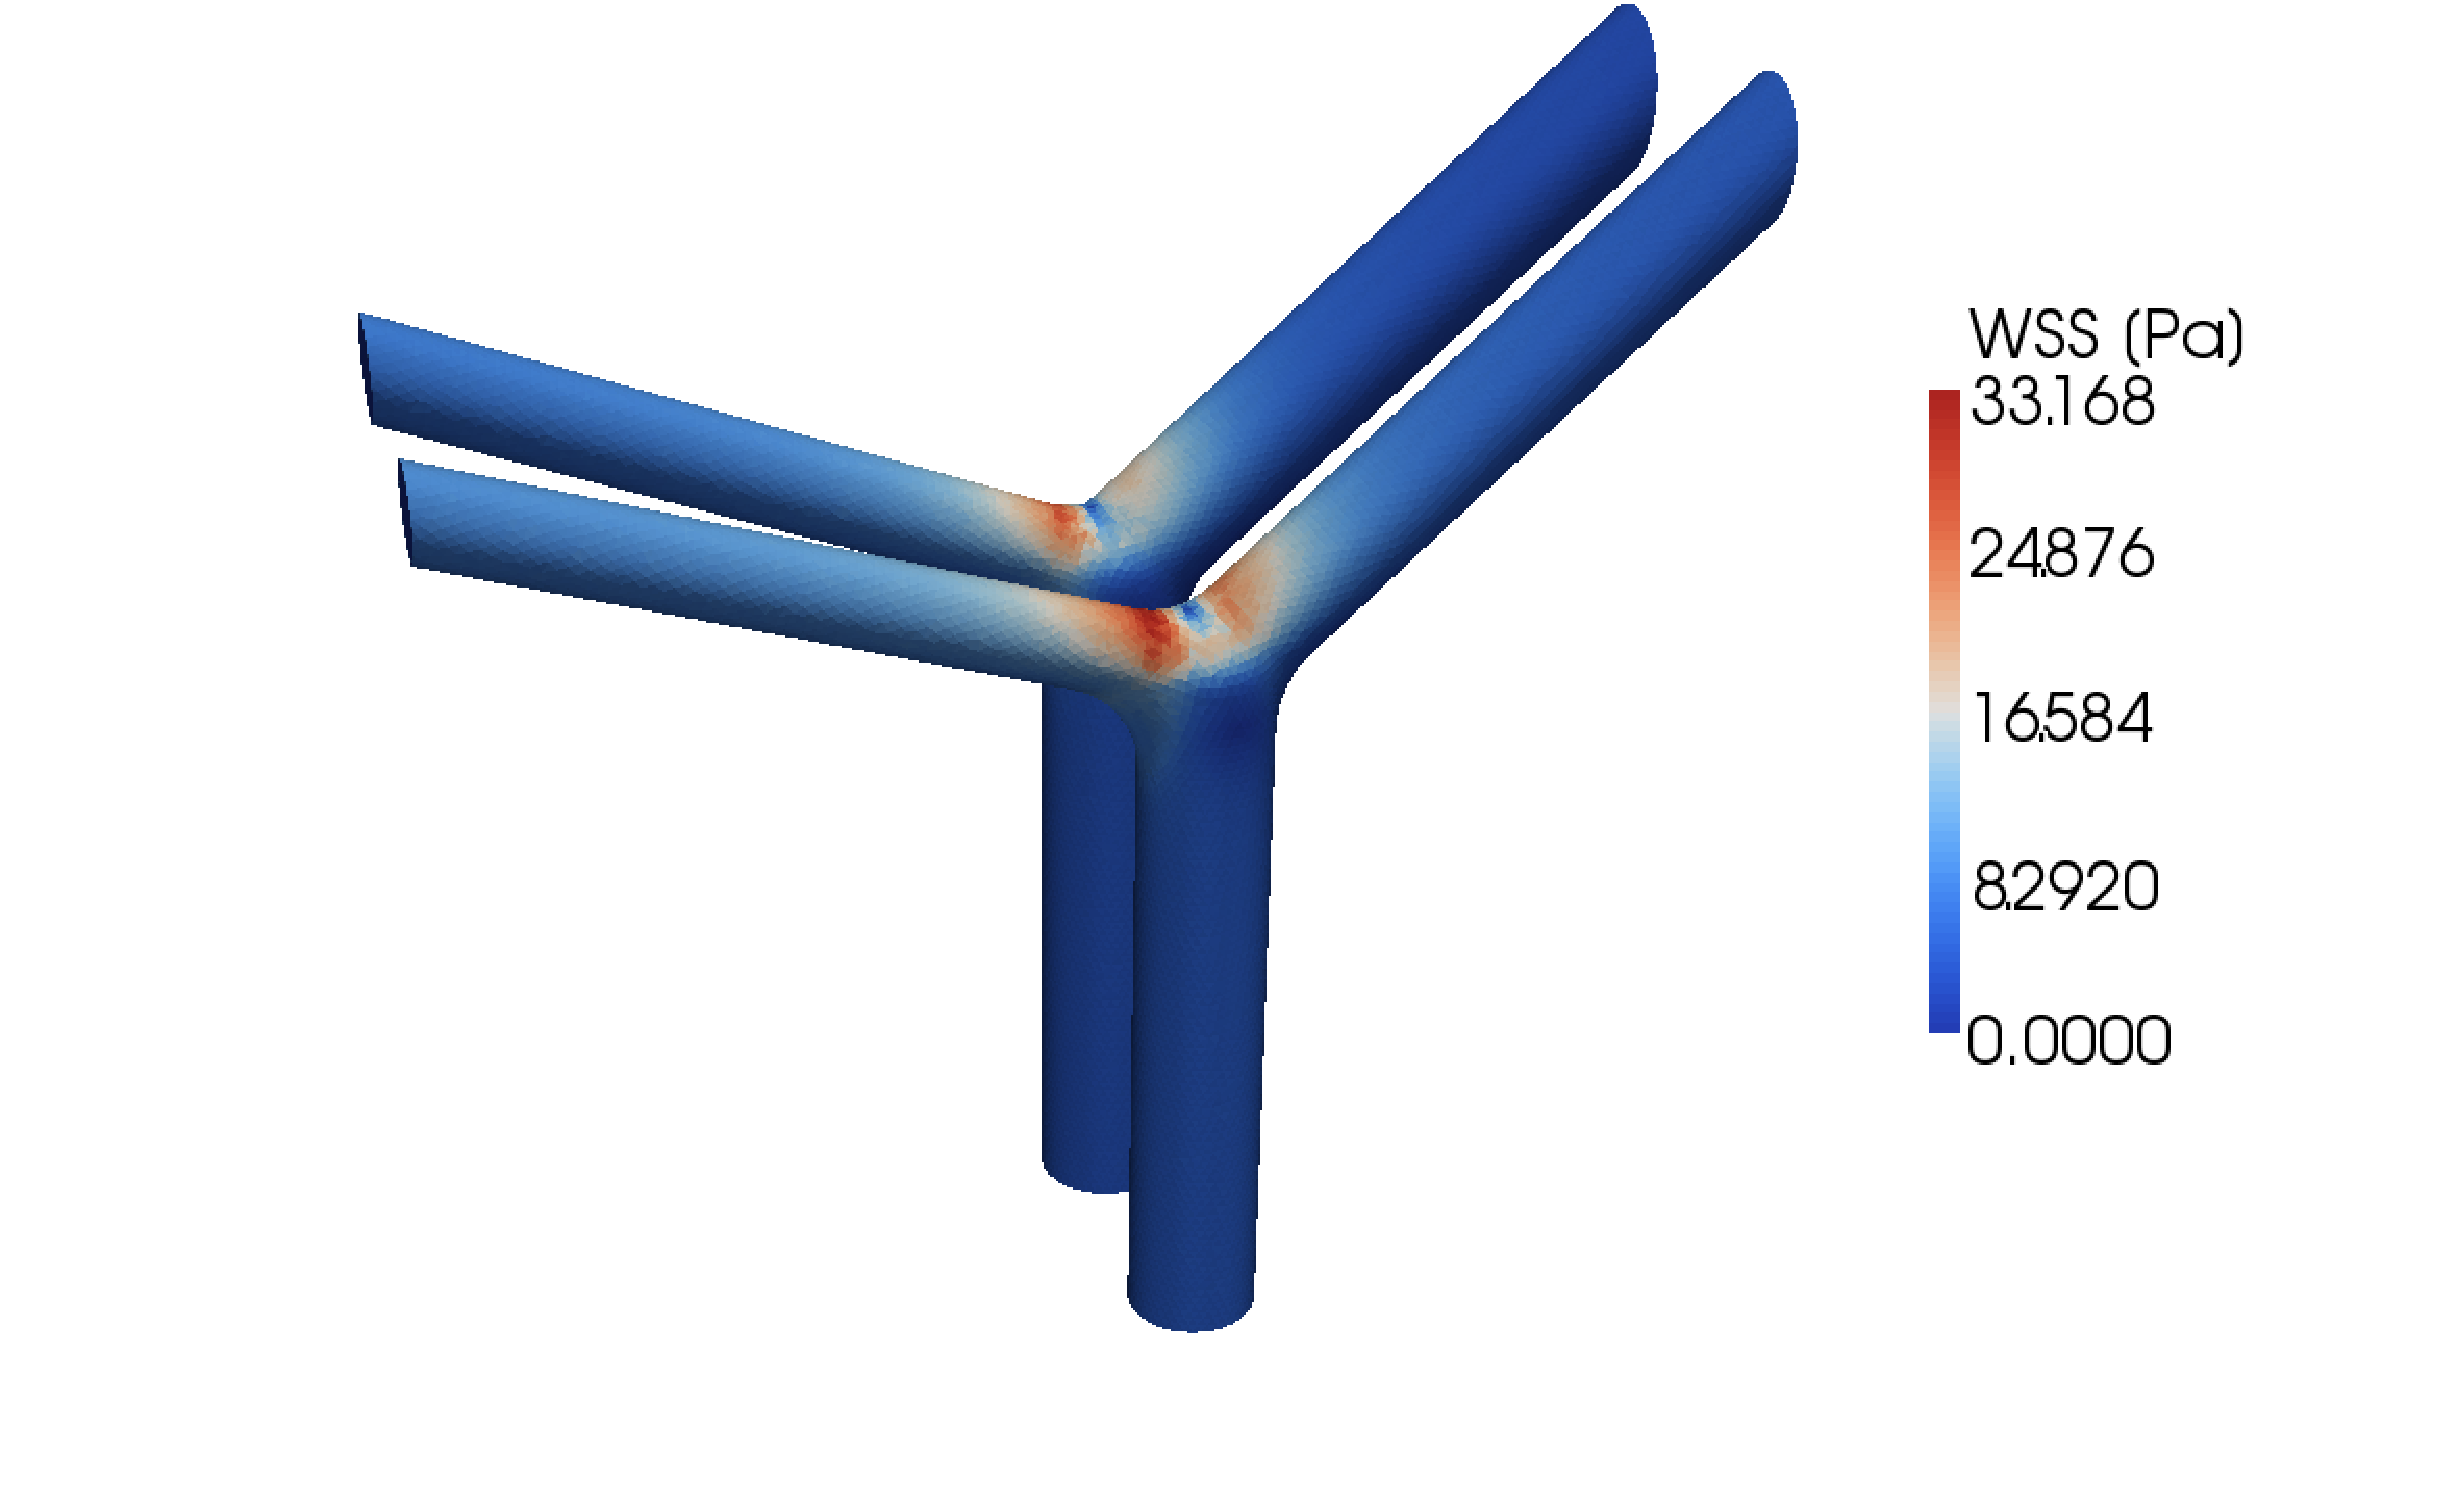
\includegraphics[width=\largefig]{chapters/kvs-2/pdf/mcas_wss_II4.pdf}
  \caption{Resulting wall shear stress in the male and female MCA
    bifurcations. Female bifurcation in front.}
  \label{fig:kvs-2:mca_wss_res}
\end{figure}

\begin{figure}
\bwfig
  \centering
  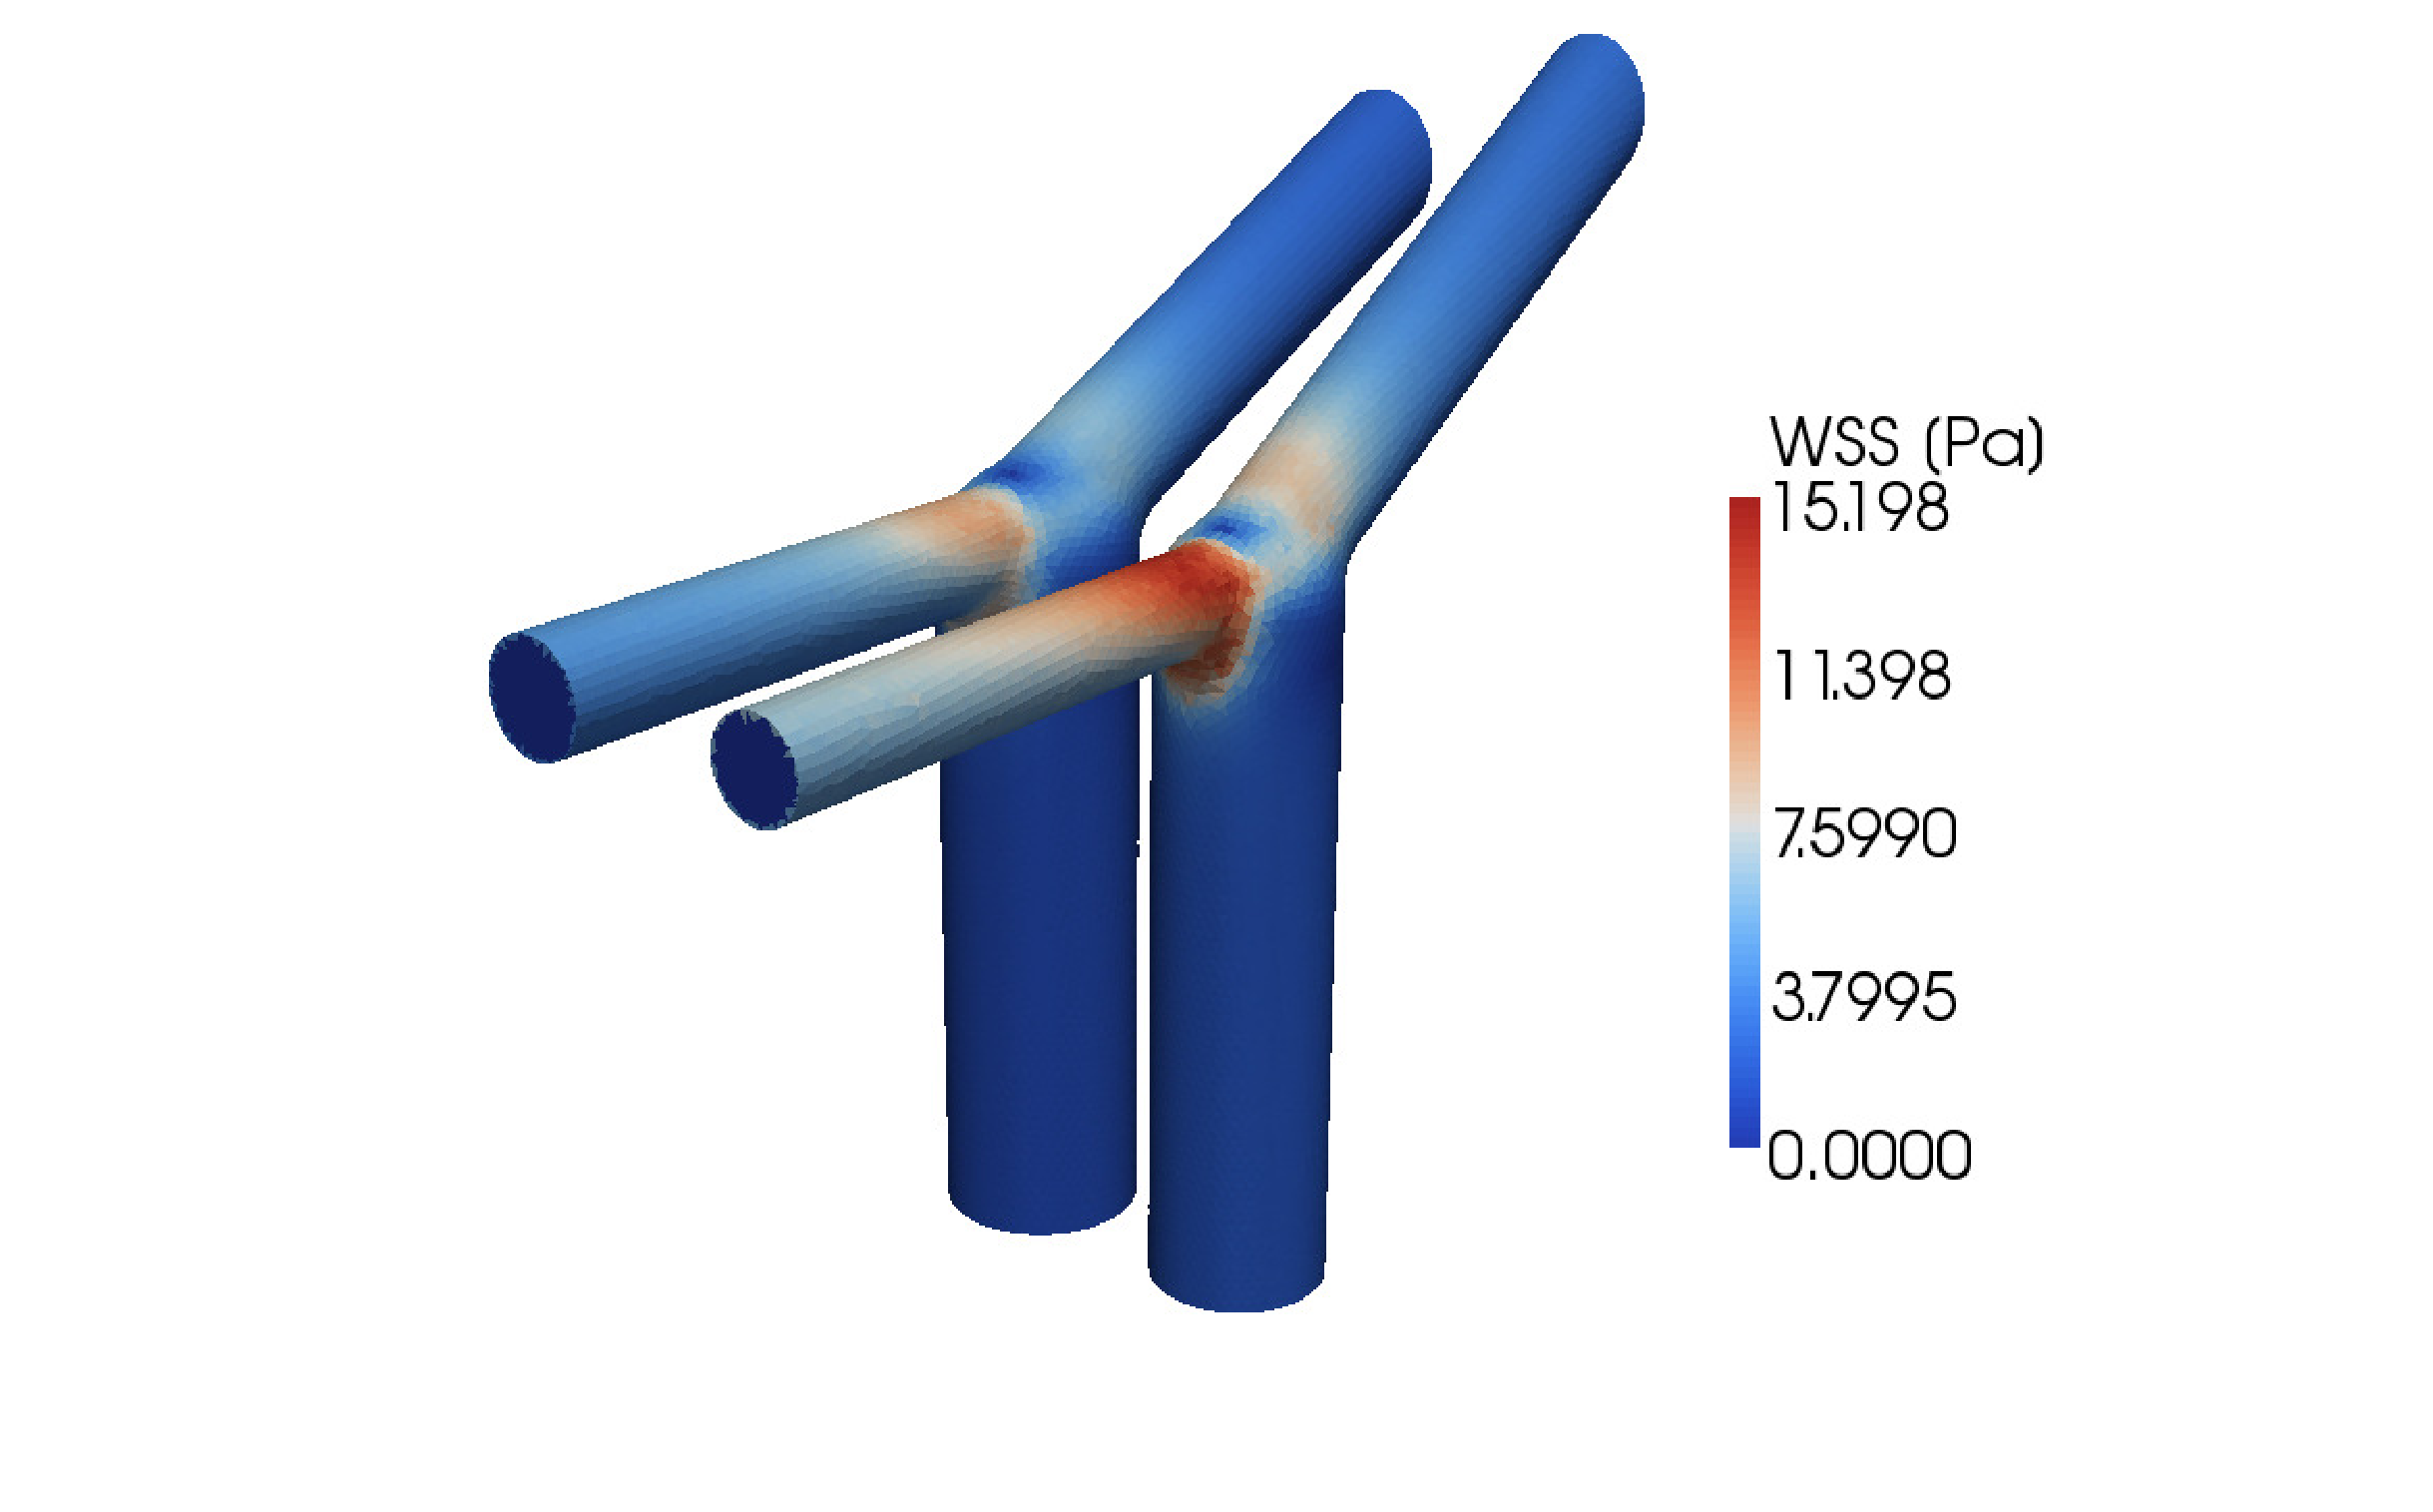
\includegraphics[width=\largefig]{chapters/kvs-2/pdf/icas_wss.pdf}
  \caption{Resulting wall shear stress in the male and female ICA
    bifurcations. Female bifurcation in front.}
  \label{fig:kvs-2:ica_wss_res}
\end{figure}

%------------------------------------------------------------------------------
\section{CFD versus 4D PC MRA in an experimental canine aneurysm} \label{dog_study}

In another study, see \citet{JiangJohnsonValen-SendstadEtAl2010}, we
quantitatively compared CFD, assuming Newtonian flow with rigid walls,
with four-dimensional Phase Contrast Magnetic Resonance Angiography
(PC MRA) techniques. The intention was both to verify the
computational techniques for creating patient-specific models and
corresponding CFD results and to understand and quantify the accuracy
of the simplest possible flow model against state-of-the-art
measurements.

Four-dimensional PC MRA is a noninvasive technique to measure flow in
the vascular system. The image acquisition consists of a scan time of
roughly 8 minutes. The canine had an average heart rate of 101 beats
per minute, and the obtained images were averaged over 808 heart
cycles. There is naturally no guarantee for a constant heart beat in
the canine, which is a source for errors. Still, errors in
the overall velocities have been shown to
be of the order of 3-10\% in large arteries such as the human pulmonary arteries;
see \citet{LotzMeierLeppertEtAl2002,EvansIwaiGristEtAl1993}, and
the accuracy of the measurements are therefore judged to be acceptable
for clinical use.

The resolution is coarse in both space and time, and the computation of
forces such as WSS might thus be difficult. In addition to this, there
might be locations in the vascular system where stenosis or plaque is
present and the quality of the 4D PC MRA might be poor. These are also
often the spots of most interest. In many cases, there are also
problems with the Velocity Encoding Sensitivity (VENC) which may
produce noise and useless data. The VENC may be adjusted to capture a
velocity within a specific range. However, less accurate data is
obtained for a wide VENC and vice versa.

\subsection{Phase contrast magnetic resonance angiography}

To test the above mentioned techniques in a complex case, our
collaborators at the Wisconsin Institutes for Medical
Research\footnote{\url{http://www.med.wisc.edu/wimr/}} created an
artificial saccular aneurysm in a carotid bifurcation of a canine
according to \citet{GermanBlack1965}. The inlet diameter was
$3.2\,\mathrm{mm}$, the height $9.4\,\mathrm{mm}$, the width
$4.3\,\mathrm{mm}$, the volume $254.3\,\mathrm{mm}^3$, the ostium area
$17.10\,\mathrm{mm}^2$, and the aspect ratio $2.18$, where the aspect
ratio is defined as the ratio between the aneurysm height and the neck
width.

Three weeks after the artificial aneurysm was created, the canine was
anesthetized and subjected to 4D PC MRA imaging studies; that is, the
velocity measurements were performed. The raw data from the 4D PC MRA
scan measurements are shown in Figure~\ref{fig:kvs-2:mass_dog} where
each solid line represents the sum of fluxes at different cross
sections of the inlet and outlet arteries. The picture to the left in
Figure~\ref{fig:kvs-2:mass_dog} shows the sum of velocities at the
inlet, which is one artery, while the picture to the right shows the
output flux; that is, the sum of the outflow in both outflow
arteries. For a more thorough description, we refer
to \citet{JiangJohnsonValen-SendstadEtAl2010}.  The coarse data
obtained from 4D PC MRA is shown in the left and middle images of
Figure~\ref{fig:kvs-2:dog_mri}, while the corresponding CFD simulation
is shown to the right.

\begin{figure}
\bwfig
  \centering
  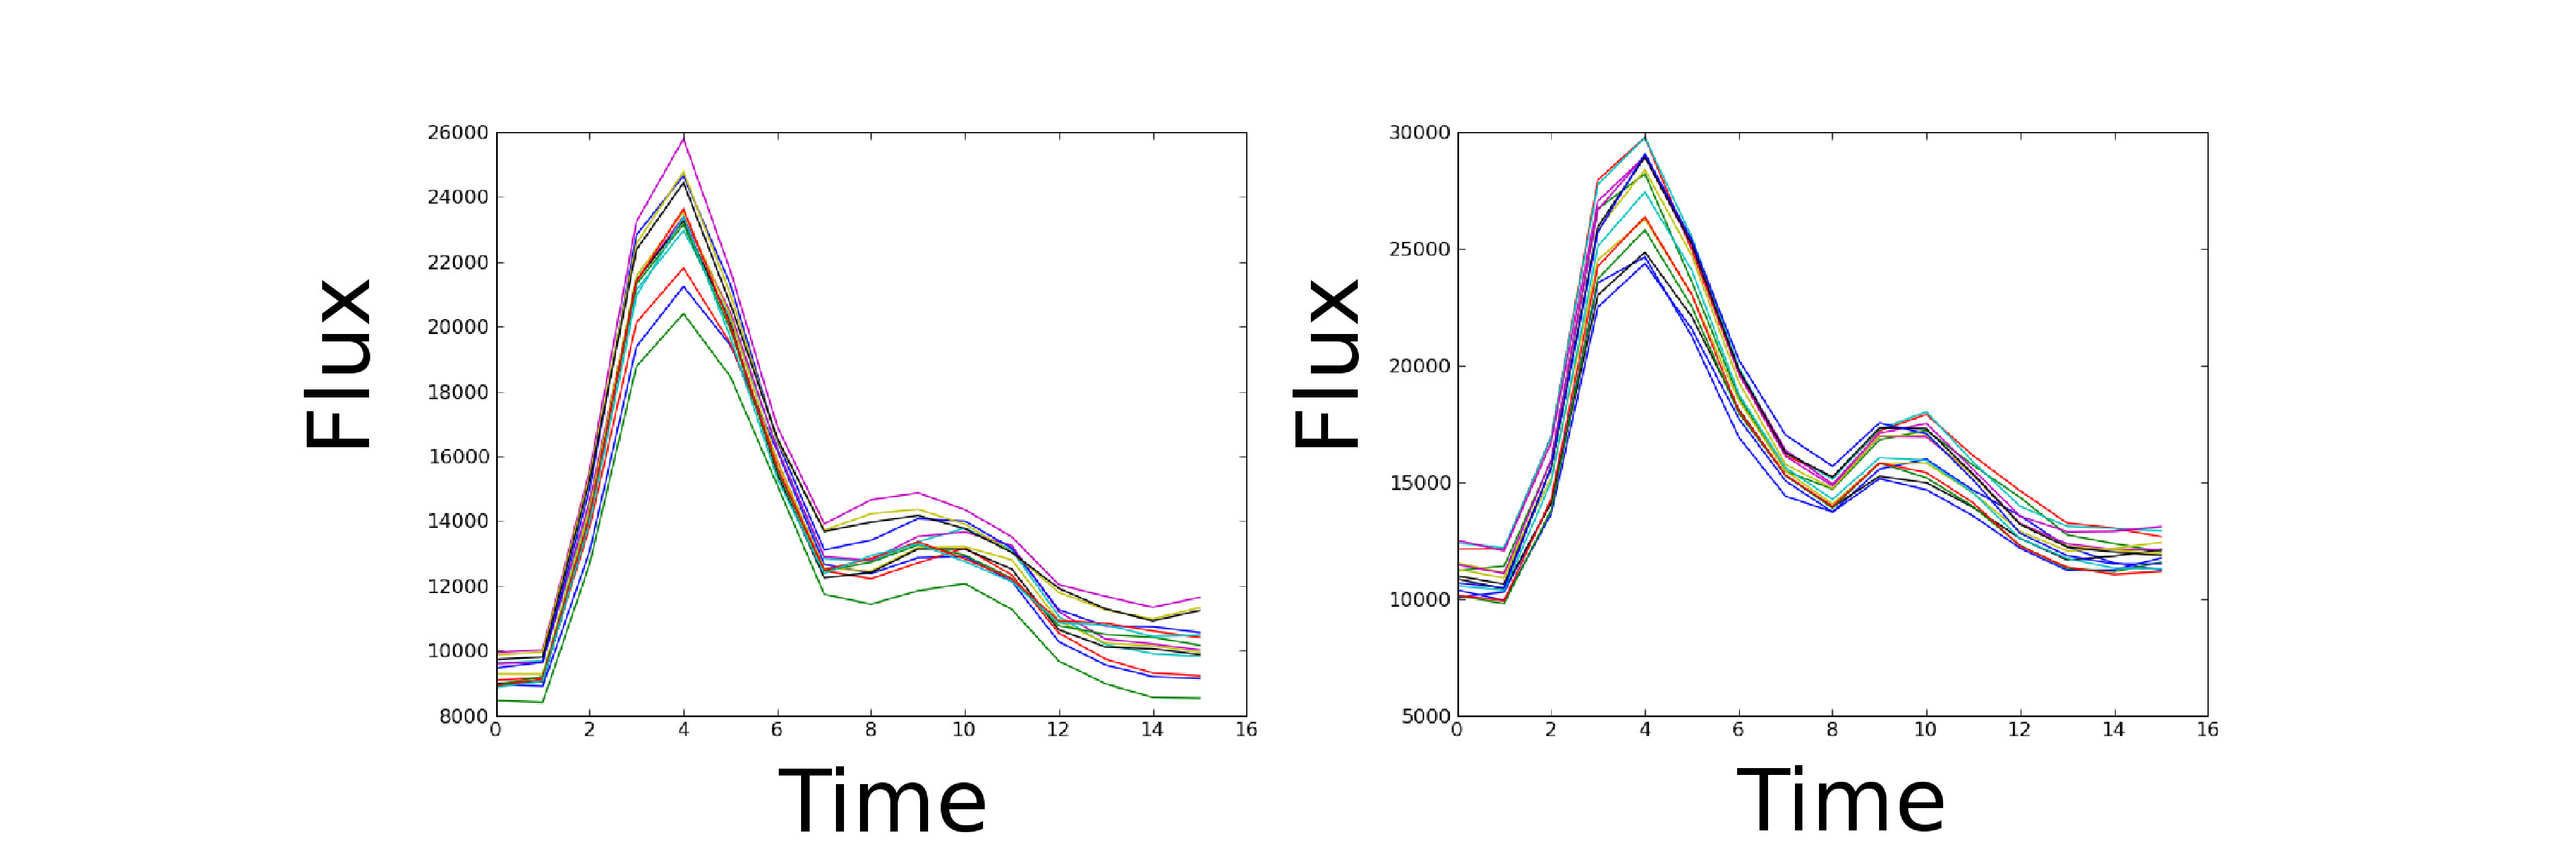
\includegraphics[width=\largefig]{chapters/kvs-2/pdf/mass_dog.pdf}
  \caption{The figure shows the raw data obtained from the 4D PC MRA scan,
    which is phase averaged from 808 heart cycles. Each line corresponds to
    the sum of fluxes obtained from a cut plane in the vertical direction.
    Measurements of mass flow differ by up to ca.~20\% between
    inlet (left) and outlet (right) in a canine. The $x$-axis shows
    the time step number.}
  \label{fig:kvs-2:mass_dog}
\end{figure}

\begin{figure}
  \centering
  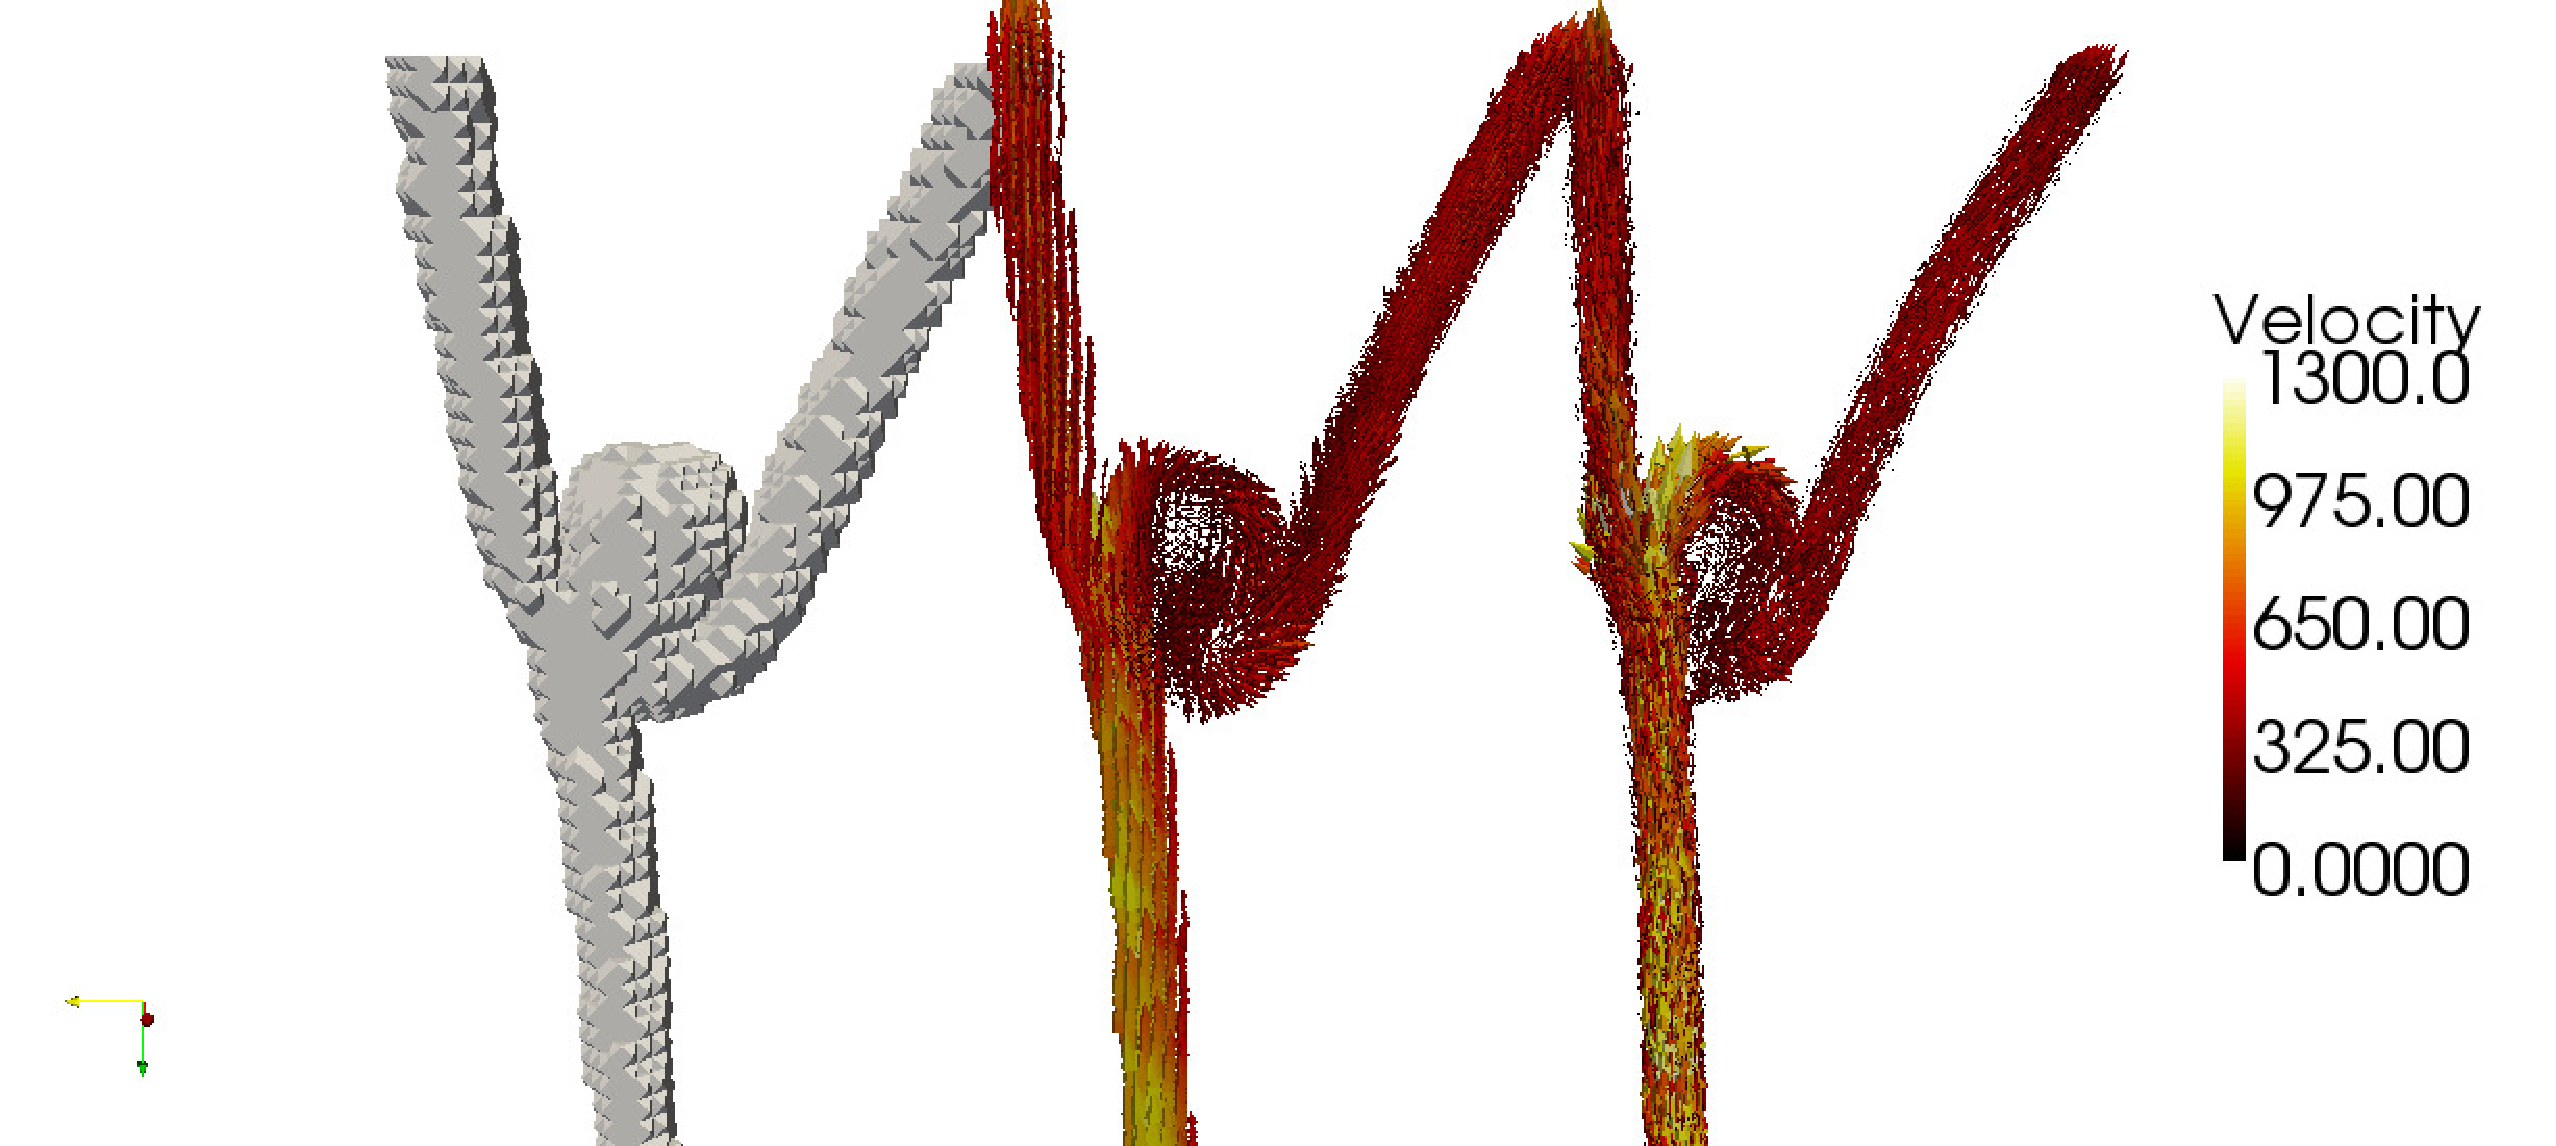
\includegraphics[width=\largefig]{chapters/kvs-2/pdf/dog_data_mr_cfd.pdf}
  \caption{Figure showing resolution of data points where velocity
    measurements are made (left), velocity measurements from 4D PC MRA
    (middle), and CFD simulations (right).}
  \label{fig:kvs-2:dog_mri}
\vspace*{-6pt}
\end{figure}

\subsection{Computational fluid dynamics}

The geometry was generated according to the procedure described in
Section~\ref{vmtk}. We solved the incompressible Navier--Stokes
equations using an Incremental Pressure Correction Scheme (IPCS) as
described in Chapter~\ref{chap:kvs-1}. We used first order elements
for both velocity and pressure, simulated over four heart beats, and
obtained the results from the last cycle. With a CFL number of roughly
ten, the number of time steps was 696 per cardiac cycle. As inflow
boundary conditions, we used an average value from the five lowermost
voxels (3D pixels / samples from the measurements) in the
$z$-direction. For the outflow, we applied a resistance boundary
condition as described in section ~\ref{resistance_bcs}. The inflow
was calculated according to Figure~\ref{fig:kvs-2:inflow_codeI} and
Figure~\ref{fig:kvs-2:inflow_codeII}.

Figure~\ref{fig:kvs-2:inflow_codeI} shows how the values in
Figure~\ref{fig:kvs-2:mass_dog} are returned as a spline function. The
factor \emp{(133.0/256)**-2} scales the voxel size to the matrix size,
so that the focus of the image corresponds to the actual size in
millimeters. The \emp{t} variable is the end time, and the scalar
$0.037$ is the equally spaced times of where measurements for \emp{v}
were made.

\begin{figure}
\bwfig
\begin{python}
def makeIC():
    Area = 8.04
    v = array([10939.45, 10714.00, 15406.95,
               25181.50, 27844.85, 24344.80,
               19578.05, 16479.55, 15168.80,
               16878.40, 16700.55, 15118.90,
               13032.50, 12121.65, 11885.90,
               11943.60, 10939.45 ]) \
                     / (Area*(133.0/256)**-2)

    t = 0.037*arange(len(v))
    t_period = 0.037*16
    return splrep(t, v), t_period
\end{python}
\caption{Measured values used for spline representation of the inflow.}
\label{fig:kvs-2:inflow_codeI}
\vspace*{-12pt}
\end{figure}

In Figure~\ref{fig:kvs-2:inflow_codeII}, a call is made to generate a spline
representation of the velocity in time by calling \emp{makeIC()}.
Then, in \emp{eval\_data}, \emp{n} is the outward facing facet normal
and \emp{t} is the time. The variable \emp{val} is a spline evaluation
such that the pulse goes in a continued cycle as time exceeds one
heart beat. Finally, each component of the velocity vector, e.g.,
\emp{values[0]}, is given the component-wise negative value of \emp{n}
(to create a flow going into the domain) times the velocity value
corresponding to the current time.

\begin{figure}
\bwfig
\begin{python}
class InflowBoundaryValue(Expression):

    def init(self, problem=None):
        self.problem = problem
        self.bc_func, self.t_period = makeIC()

    def eval_cell(self, values, x, ufc_cell):

        # Create DOLFIN Cell
        cell = Cell(mesh, ufc_cell.index)

        # Get normal for current facet
        assert(ufc_cell.local_facet >= 0)
        n = cell.normal(ufc_cell.local_facet)

        # Compute boundary value
        t = self.problem.t
        val = splev(t - int(t/self.t_period)*self.t_period,
                    self.bc_func)
        values[0] = -n.x()*val
        values[1] = -n.y()*val
        values[2] = -n.z()*val

    def value_shape(self):
        return (3,)
\end{python}
\caption{Calculation of inflow boundary value for the velocity.}
\label{fig:kvs-2:inflow_codeII}
\end{figure}

\enlargethispage{10pt}

\vspace*{-10pt}

\subsection{Results}

The resulting velocity field from 4D PC MRA and CFD calculations
during peak systole are shown in Figure~\ref{fig:kvs-2:dog_mri}, and
illustrates an overall good agreement between CFD and 4D PC MRA. For
both canines (only one shown here), we obtained a similarity of more
than 70\% with respect to the velocity but only 22-31\% similarity
with respect to the WSS. For further details, we refer
to \citet{JiangJohnsonValen-SendstadEtAl2010}.

\subsection{Discussion}

The reason for using the average values of the five lowermost cross
sections as inflow is that given the resolution of the 4D PC MRA, each
level of voxels is not\vadjust{\pagebreak} necessarily mass conserving. As seen in
Figure~\ref{fig:kvs-2:mass_dog}, the sum of mass in a plane may vary
by as much as 20\% between sections (the solid lines).
It is also clearly visible in this figure that peak systole appears at
time step four in both left (inflow) and right (outflow) image of the
figure, but the ``bump'' at mid deceleration has shifted from time
step seven at the inflow to eight at the outflow.  This may be because
of the so-called Windkessel effect, which may only be captured using a
fluid--structure interaction model, but it is difficult to conclude due
to the coarseness of the measurements.

A limitation of the current study is that the results should not be
interpreted as physiologically correct since the technique consists of
cutting off one of the ICAs and creating an artificial bifurcation
(and aneurysm) by moving the rest of the vessel over to the other
ICA. This means that one of the ICAs supplies both left and right sides
of the canine brain.

In the 4D PC MRA measurements at the left side of the parent artery in
Figure~\ref{fig:kvs-2:dog_mri}, there are no boundary layers due to
isotropic voxels, and the colors appear brighter since high velocities
are possible close to the wall.  The CFD simulations have short arrows
at the same location indicating that the boundary layer has been
resolved and we get lower velocity magnitudes.  This is an obvious
drawback with the 4D PC MRA. Thus, we get a good agreement with the
velocity measurements, but poor agreement for computed wall shear
stresses. The reason for this is believed to be the poor spatial
resolution of the 4D PC MRA data. For a more thorough description, we
refer to \citet{JiangJohnsonValen-SendstadEtAl2010}.

Each of the two methods has its strengths and weaknesses. While 4D PC
MRA is fast, cheap and harmless, it uses average values over a voxel
volume and fails to correctly compute WSS, recirculation zones, and
possible turbulent structures. It also fails to provide values where
the VENC is out of focus or in the presence of a stenosis. In
contrast, CFD is expensive but may provide accurate computations of
WSS over the entire domain.

Combined, the two methods may give a better understanding of the
importance of boundary conditions, whether or not fluid--structure
interaction is of importance, and possible pitfalls using the
different methods. A first natural extension of this study may be to
describe blood as a non-Newtonian fluid to determine whether or not
non-Newtonian effects are of importance.

%------------------------------------------------------------------------------
\section{Patient-specific Circle of Willis} \label{cok}

\subsection{Background}

In a study performed in collaboration with clinicians from the
Neuroradiology department at Riks\-hospitalet University Hospital in
Oslo, we wanted to investigate whether we are able to reproduce
velocities in a full Circle of Willis with measurements at the inflow
and compare with measurements at the outflow using resistance boundary
conditions from the
literature \citep{AlastrueyParkerPeiroEtAl2007,Vignon-ClementelFigueroaJansenEtAl2006}.
Such an evaluation or verification of boundary conditions is essential
before proceeding with more sophisticated models for the entire
intracranial vasculature.

\begin{figure}
\bwfig
  \centering
  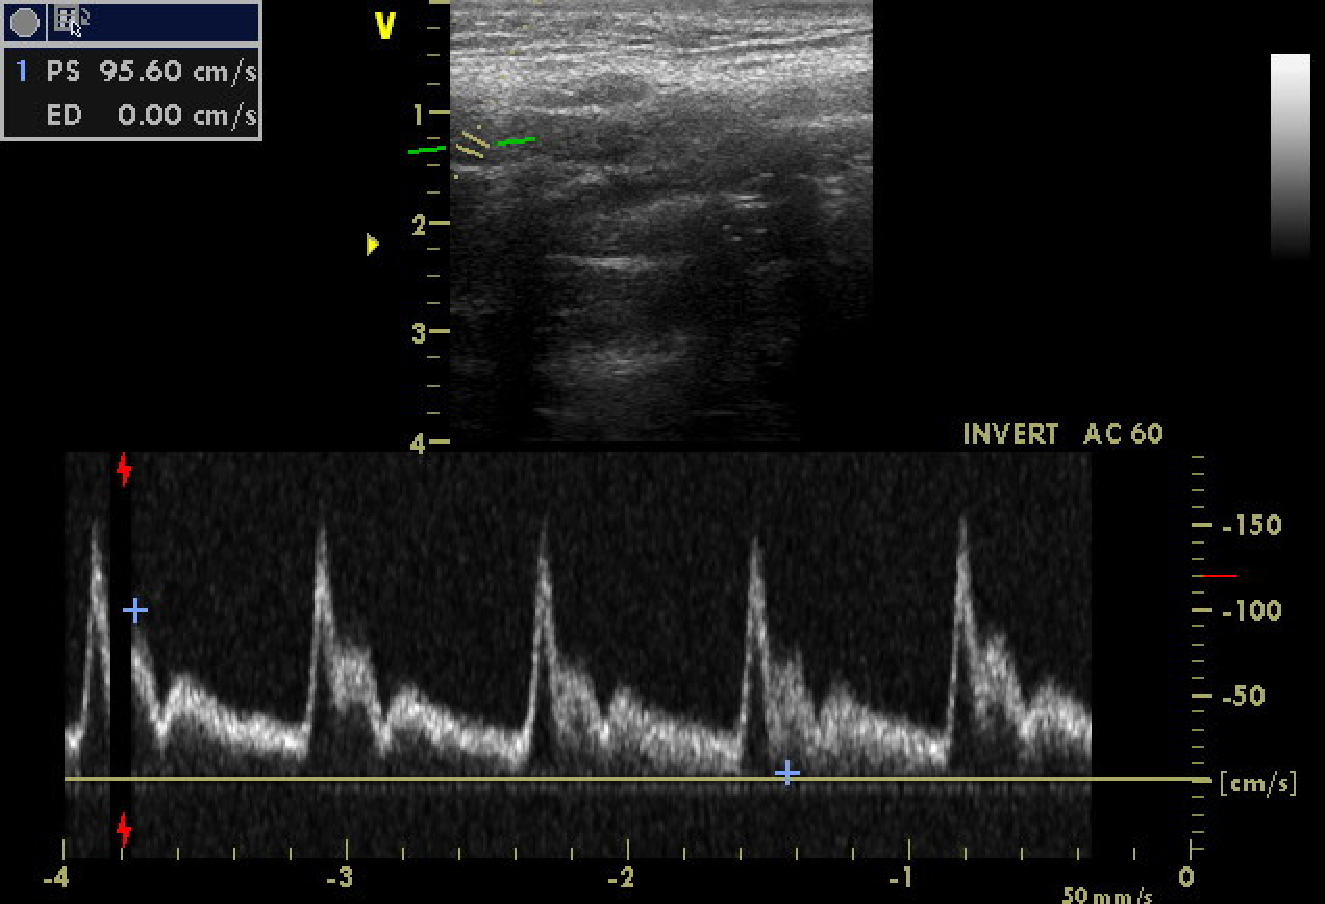
\includegraphics[width=\largefig]{chapters/kvs-2/pdf/ica.pdf} \\
  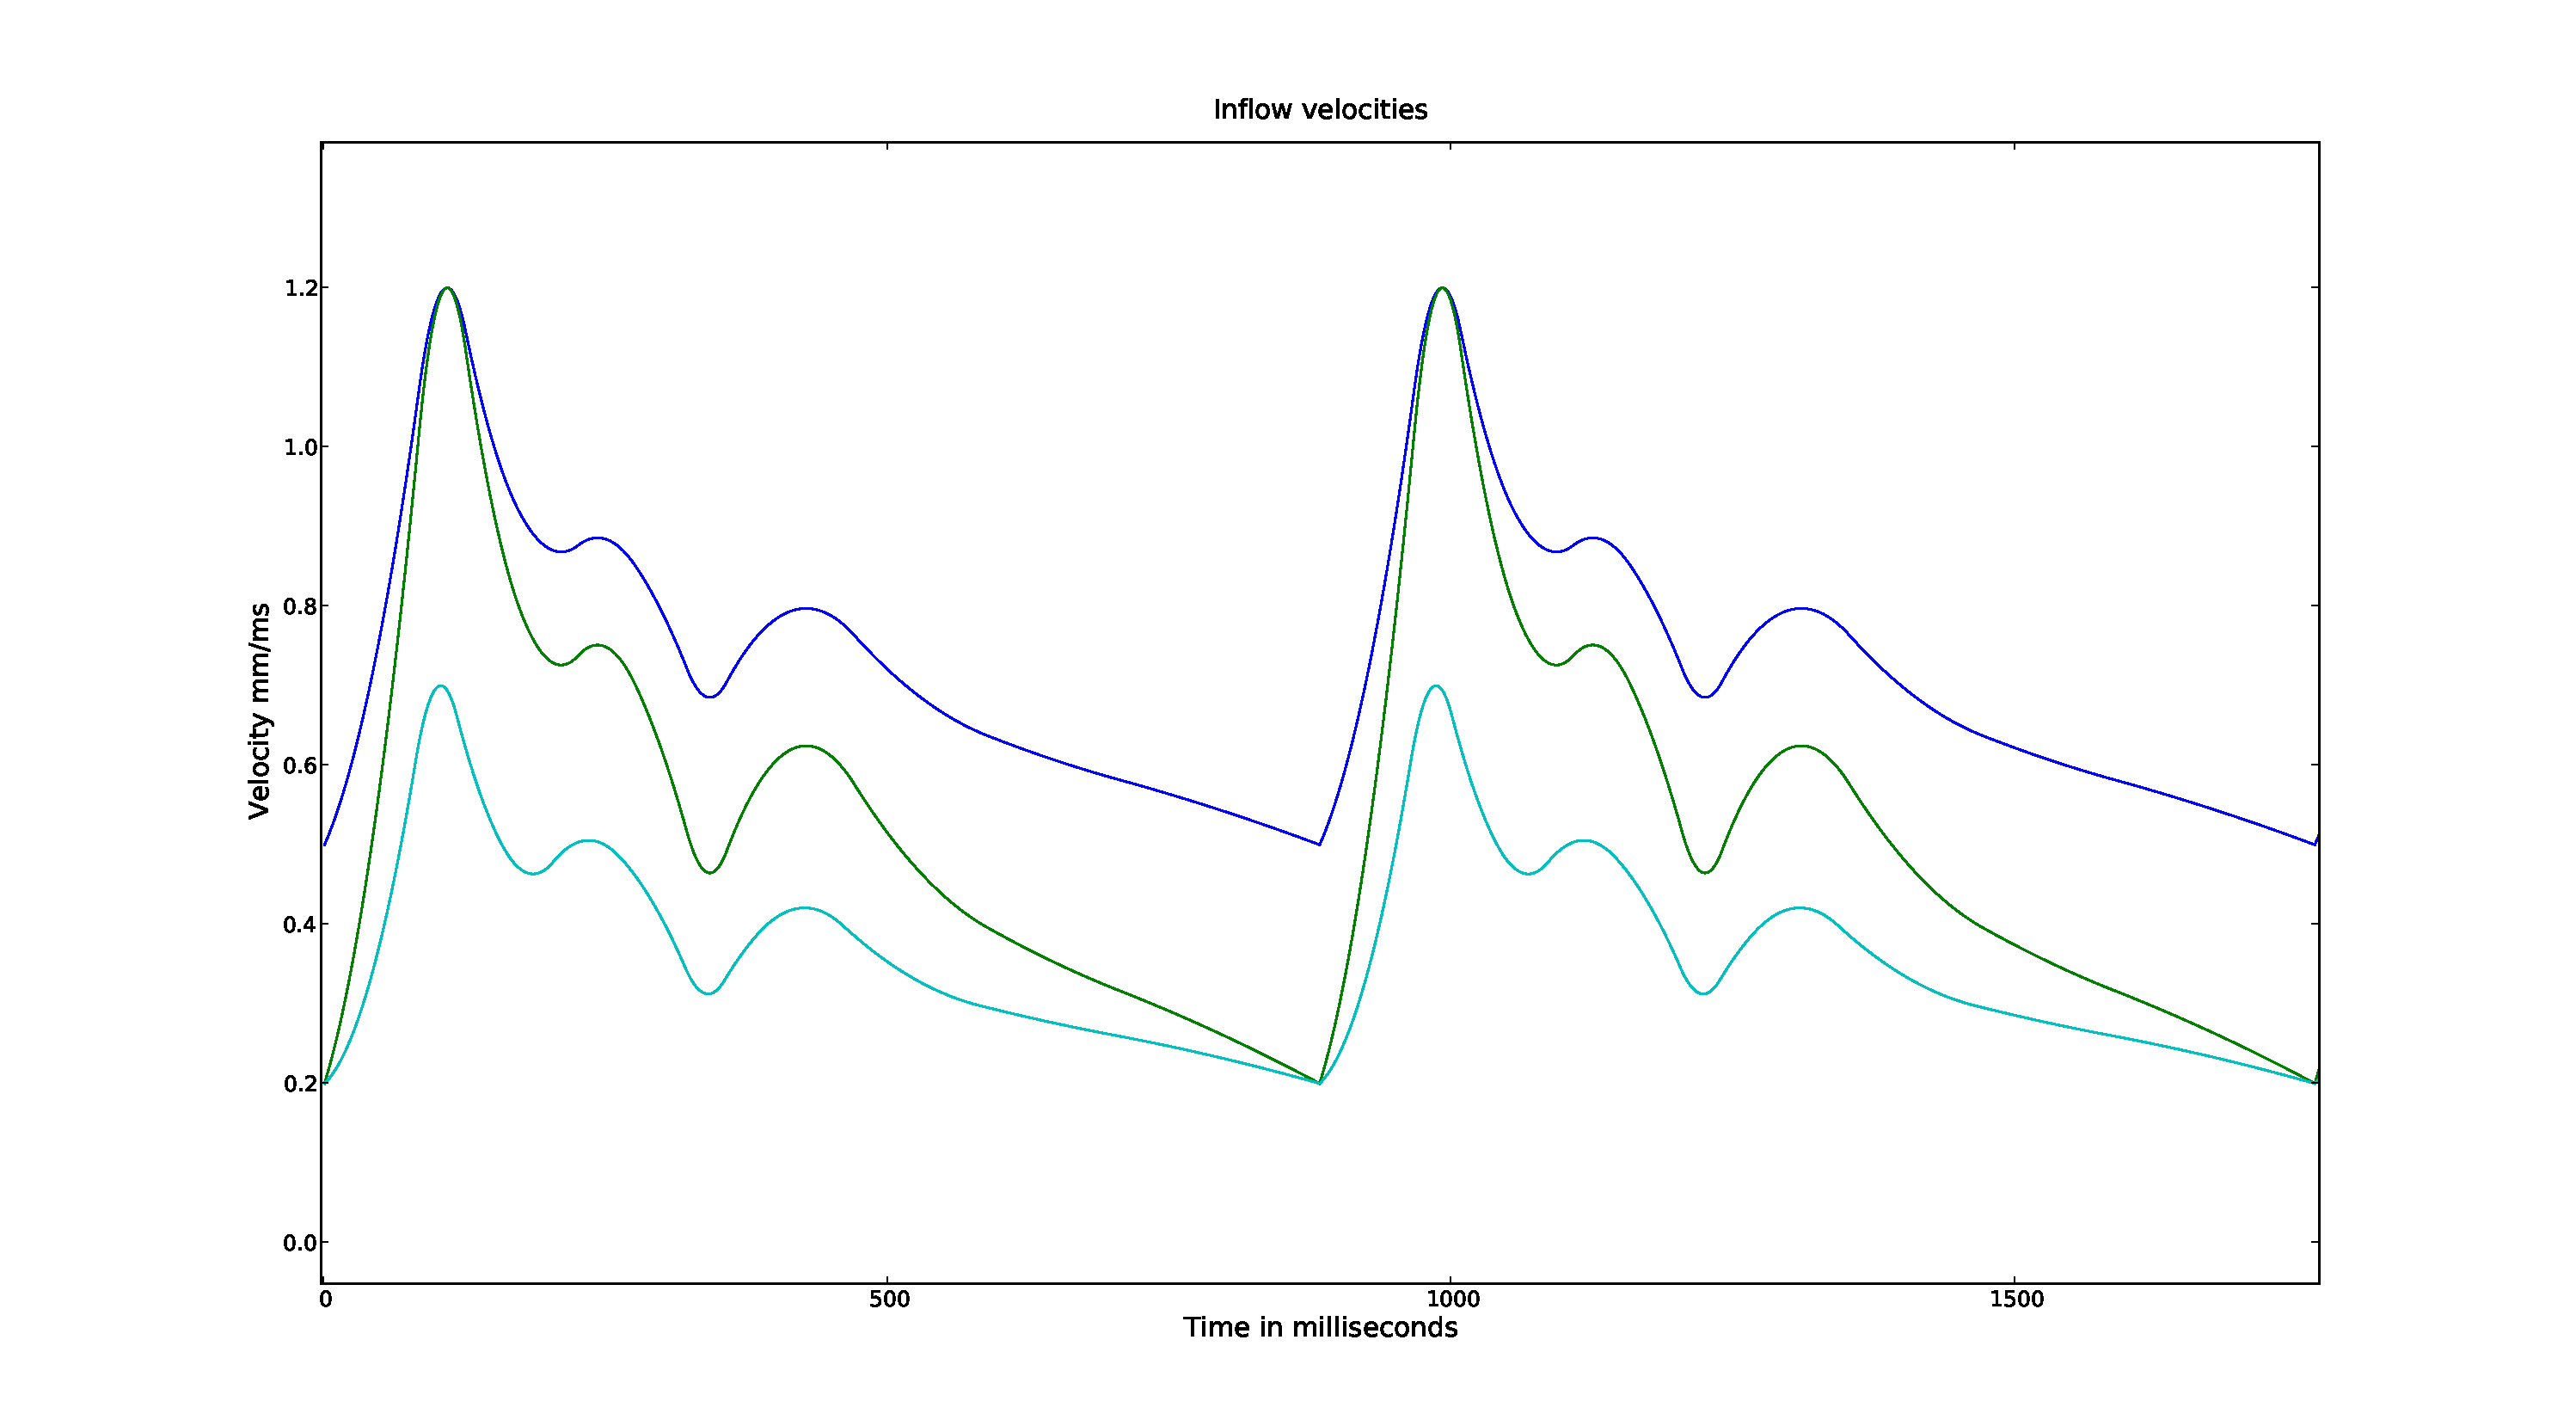
\includegraphics[width=\largefig]{chapters/kvs-2/pdf/cok_inflow.pdf}
  \caption{Inflow velocities used for the simulation of blood flow in
    a patient-specific Circle of Willis. Screenshot from TCD machine
    (top) with the artery on top and waveform below and implemented
    values (bottom). See text for details.}
  \label{fig:kvs-2:cok_inflow}
\end{figure}

\subsection{Method}

Transcranial Doppler (TCD) was performed on a healthy volunteer at
rest. During the velocity recording, the average pulse was about 73
beats per minute. The velocity measurements were used as boundary
conditions for the vessels that are the main suppliers of blood to the
brain; that is, the ICAs and VAs. Figure~\ref{fig:kvs-2:cok_inflow}
shows the resulting waveform (right) that was applied from the
measurements (left). The figure shows the ICA velocities from the top
with equal value at peak systole ($120\,\mathrm{cm}/\mathrm{s}$) and
differing at end diastole (minimum 50cm/s in right ICA and 20 cm/s in
left ICA). The lowermost line has a different waveform and shows
values for two superimposed VAs since they are equal. The vasculature
(based on an MRA scan) for this patient was already available from a
previous study performed nine months earlier. The major vessels (ICA,
MCA, PCA, ACA, VA, BA) were segmented as described in
Section~\ref{vmtk}. The simulations were performed on meshes with
three boundary layers where the number of tetrahedron cells were
approximately $400,000$, $900,000$ and $2,600,000$. We used continuous
linear elements for both velocity and pressure, and an incremental
pressure correction scheme with Adams--Bashforth implicit convection
and Crank--Nicolson diffusion to solve the incompressible
Navier--Stokes equations. The resolution in time was 3,532 time steps
per heart beat on the coarsest mesh.

\subsection{Results}

Based upon images obtained from TCD, we compare only one point in
time: peak systole. Since there is a large difference in the sum of
inflow areas and outflow areas, we consider only the flow division
between the arteries compared to measurements.
Table~\ref{measure_vs_comp} shows the measured and calculated
velocities for the major arteries.

\begin{table}
  \centering
  \begin{tabular}{ccccc}
    \toprule
    Artery &Measured, L&Computed, L &Measured, R&Computed, R \\
    \midrule
    MCA & 70, 120 		& 87  & 140, 150 	& 55	\\
    ACA & 200  		& 100  	& 90, 100 	& 65	\\
    PCA & 70, 80  		& 62 	& 80  		& 100  \\
    \bottomrule
  \end{tabular}
  \caption{Measured versus computed values for flow
    velocities [cm/s] at left (L) and right (R) outflow arteries in a patient-specific Circle of Willis at peak
    systole. The cells with two values refer to different measurements
    made 5~weeks apart.}
  \label{measure_vs_comp}
\end{table}

\subsection{Discussion}

The results of the current study do not match very well with measured
values. This may indicate that the type of boundary conditions applied
here may not describe the peripheral resistance properly. However,
there are many sources of error that must be considered.  First, TCD
is difficult to perform and subject to errors. Personal communication
with the neuroradiologist suggests errors at the scale of 20\%.
Second, we have no information on when peak systole appears in the
different arteries. It seems reasonable that there is a small shift in
time since the blood flows from the heart and through different
arteries before it meets in the Circle of Willis. At present, we have not been able to
quantify this shift. Third, the velocity itself may differ at
different times for various reasons. This is illustrated by the cells
containing two values in Table~\ref{measure_vs_comp}, which refer to
two measurements of the same vessel in the same person only 5 weeks
apart.

It is also a great challenge to segment the complete Circle of Willis due to great
variations in diameters. This is clearly visible when performing an
automatic segmentation where many of the smaller vessels disappear.
It is known that the BA has approximately 50 tiny vessels that are
clearly not present in Figure~\ref{fig:kvs-2:screenshot}. The reason
for this is that MRA measurements are based upon velocities, and hence
the velocities in these vessels are too small to be captured. By
calculating and summing up the in- and outflow areas using the code in
Figure~\ref{fig:kvs-2:area_code}, we actually get an area difference
of
$37.18\,\mathrm{mm}^2-25.33\,\mathrm{mm}^2=11.85\,\mathrm{mm}^2$. It
is not known what the correct area should be.

The simulations also show that it might be problematic to not include
a large fraction of the parent artery when performing simulations on a
smaller fraction of the vasculature. It is common to apply either a
flat velocity profile or a Womersley profile upstream of the location
of interest. This is clearly not the case as shown in
Figure~\ref{fig:kvs-2:cok_ica} where the flow is highly non-uniform.

\begin{figure}
\bwfig
\begin{python}
def area(self, i):
    f = Constant(1)
    A = f*ds(i)
    a = assemble(A,
                 exterior_facet_domains=self.sub_domains,
                 mesh=self.mesh)
    return a
\end{python}
\caption{Calculation of the areas of the Circle of Willis geometry.}
\label{fig:kvs-2:area_code}
\end{figure}

\begin{figure}
  \ffigbox{\caption{Patient-specific Circle of Willis (of the second author).}
           \label{fig:kvs-2:screenshot}}
          {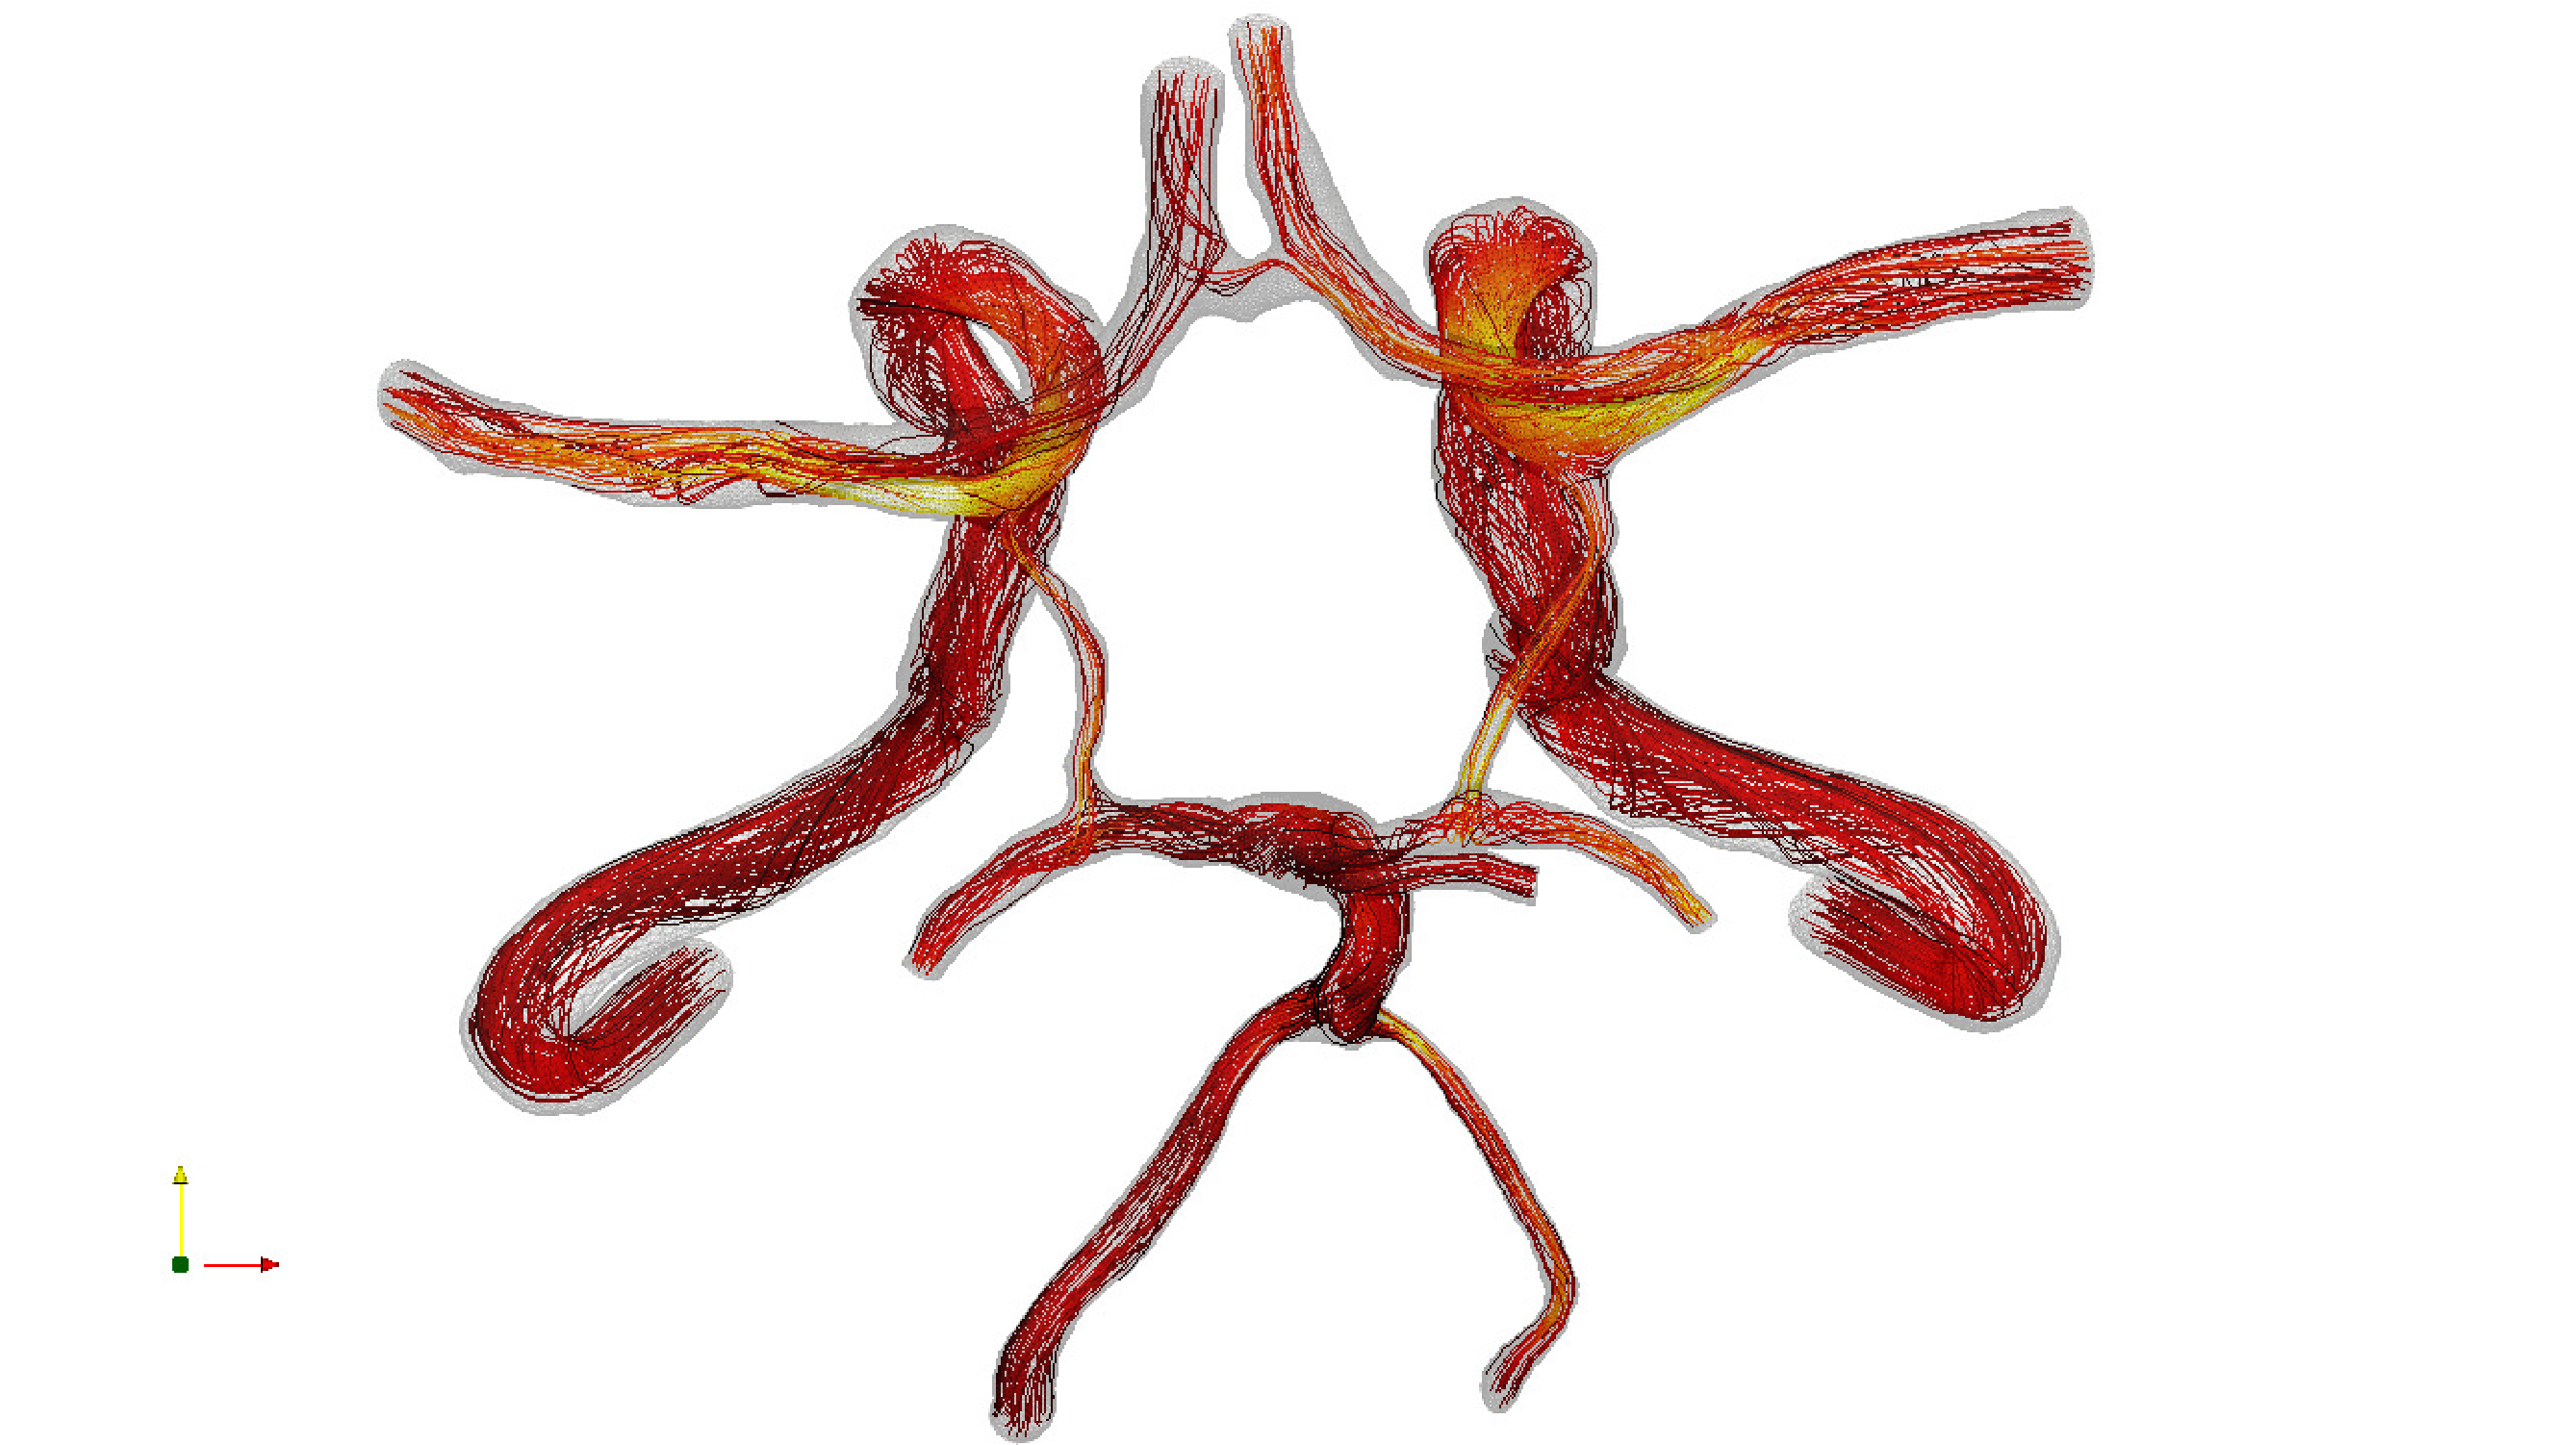
\includegraphics[width=\fullfig]{chapters/kvs-2/pdf/cok_top_steam_white.pdf}}
\end{figure}

\begin{figure}
\bwfig
  \centering
  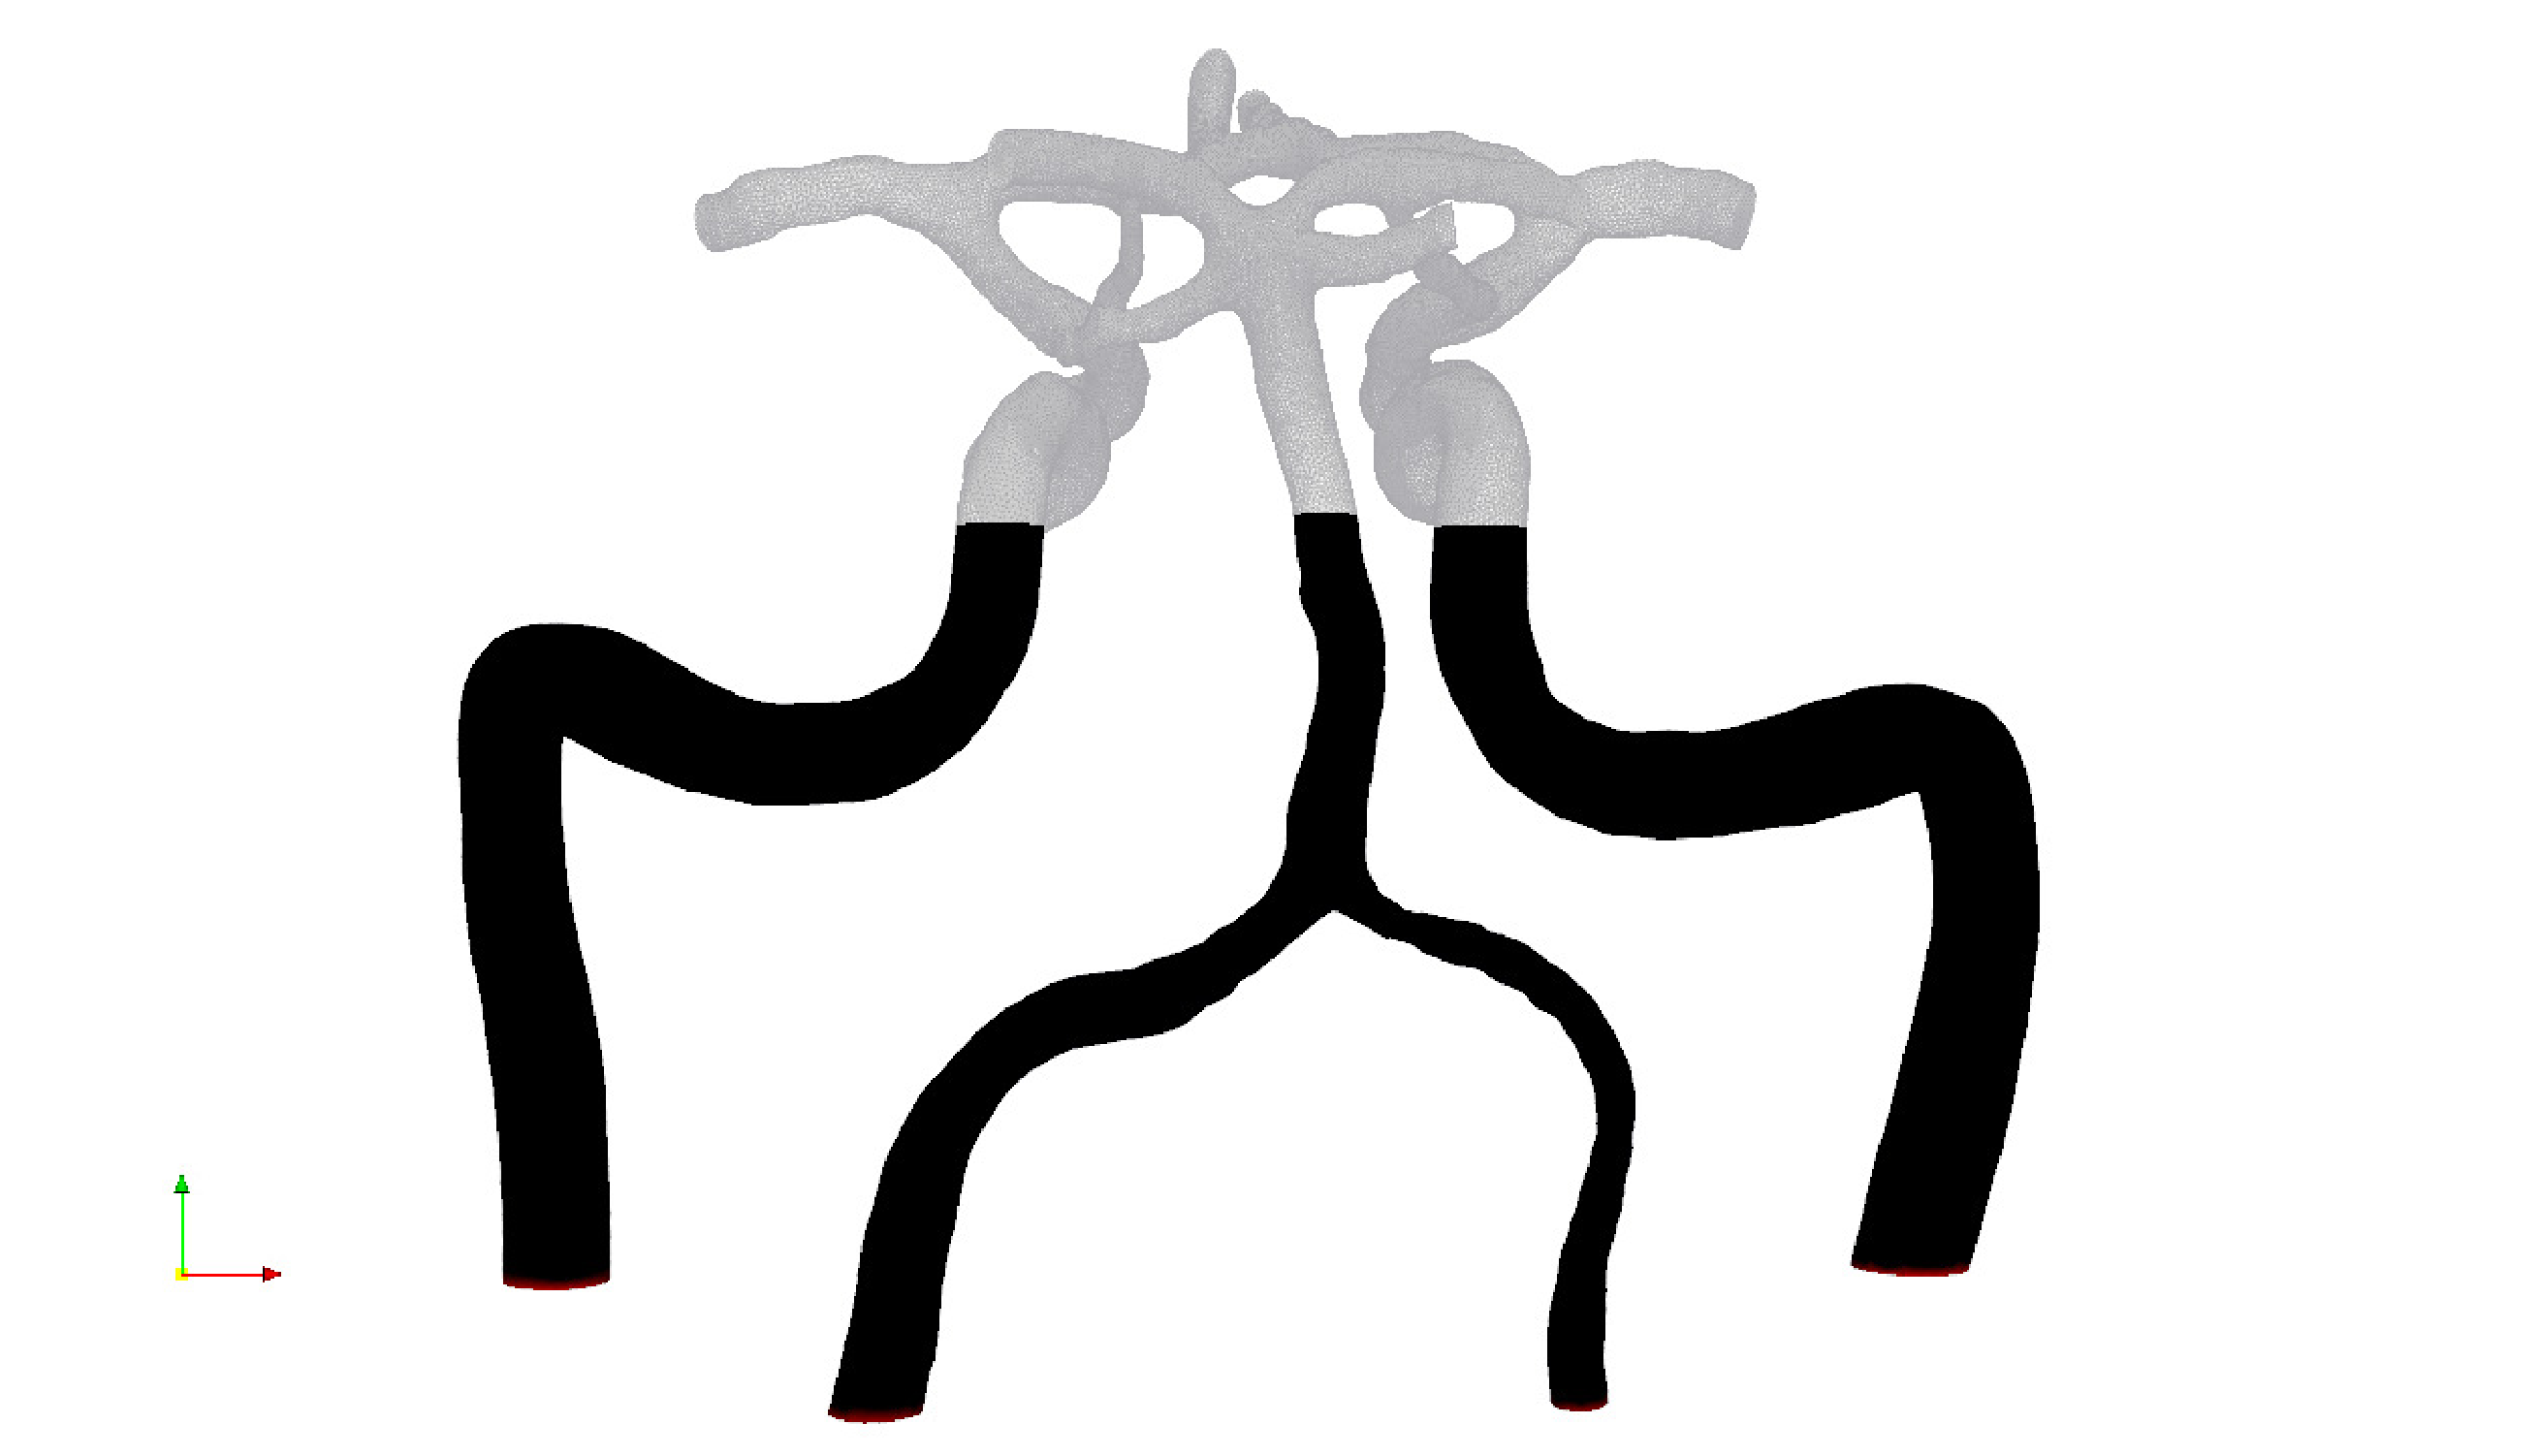
\includegraphics[width=\largefig]{chapters/kvs-2/pdf/cok_slice.pdf} \\
  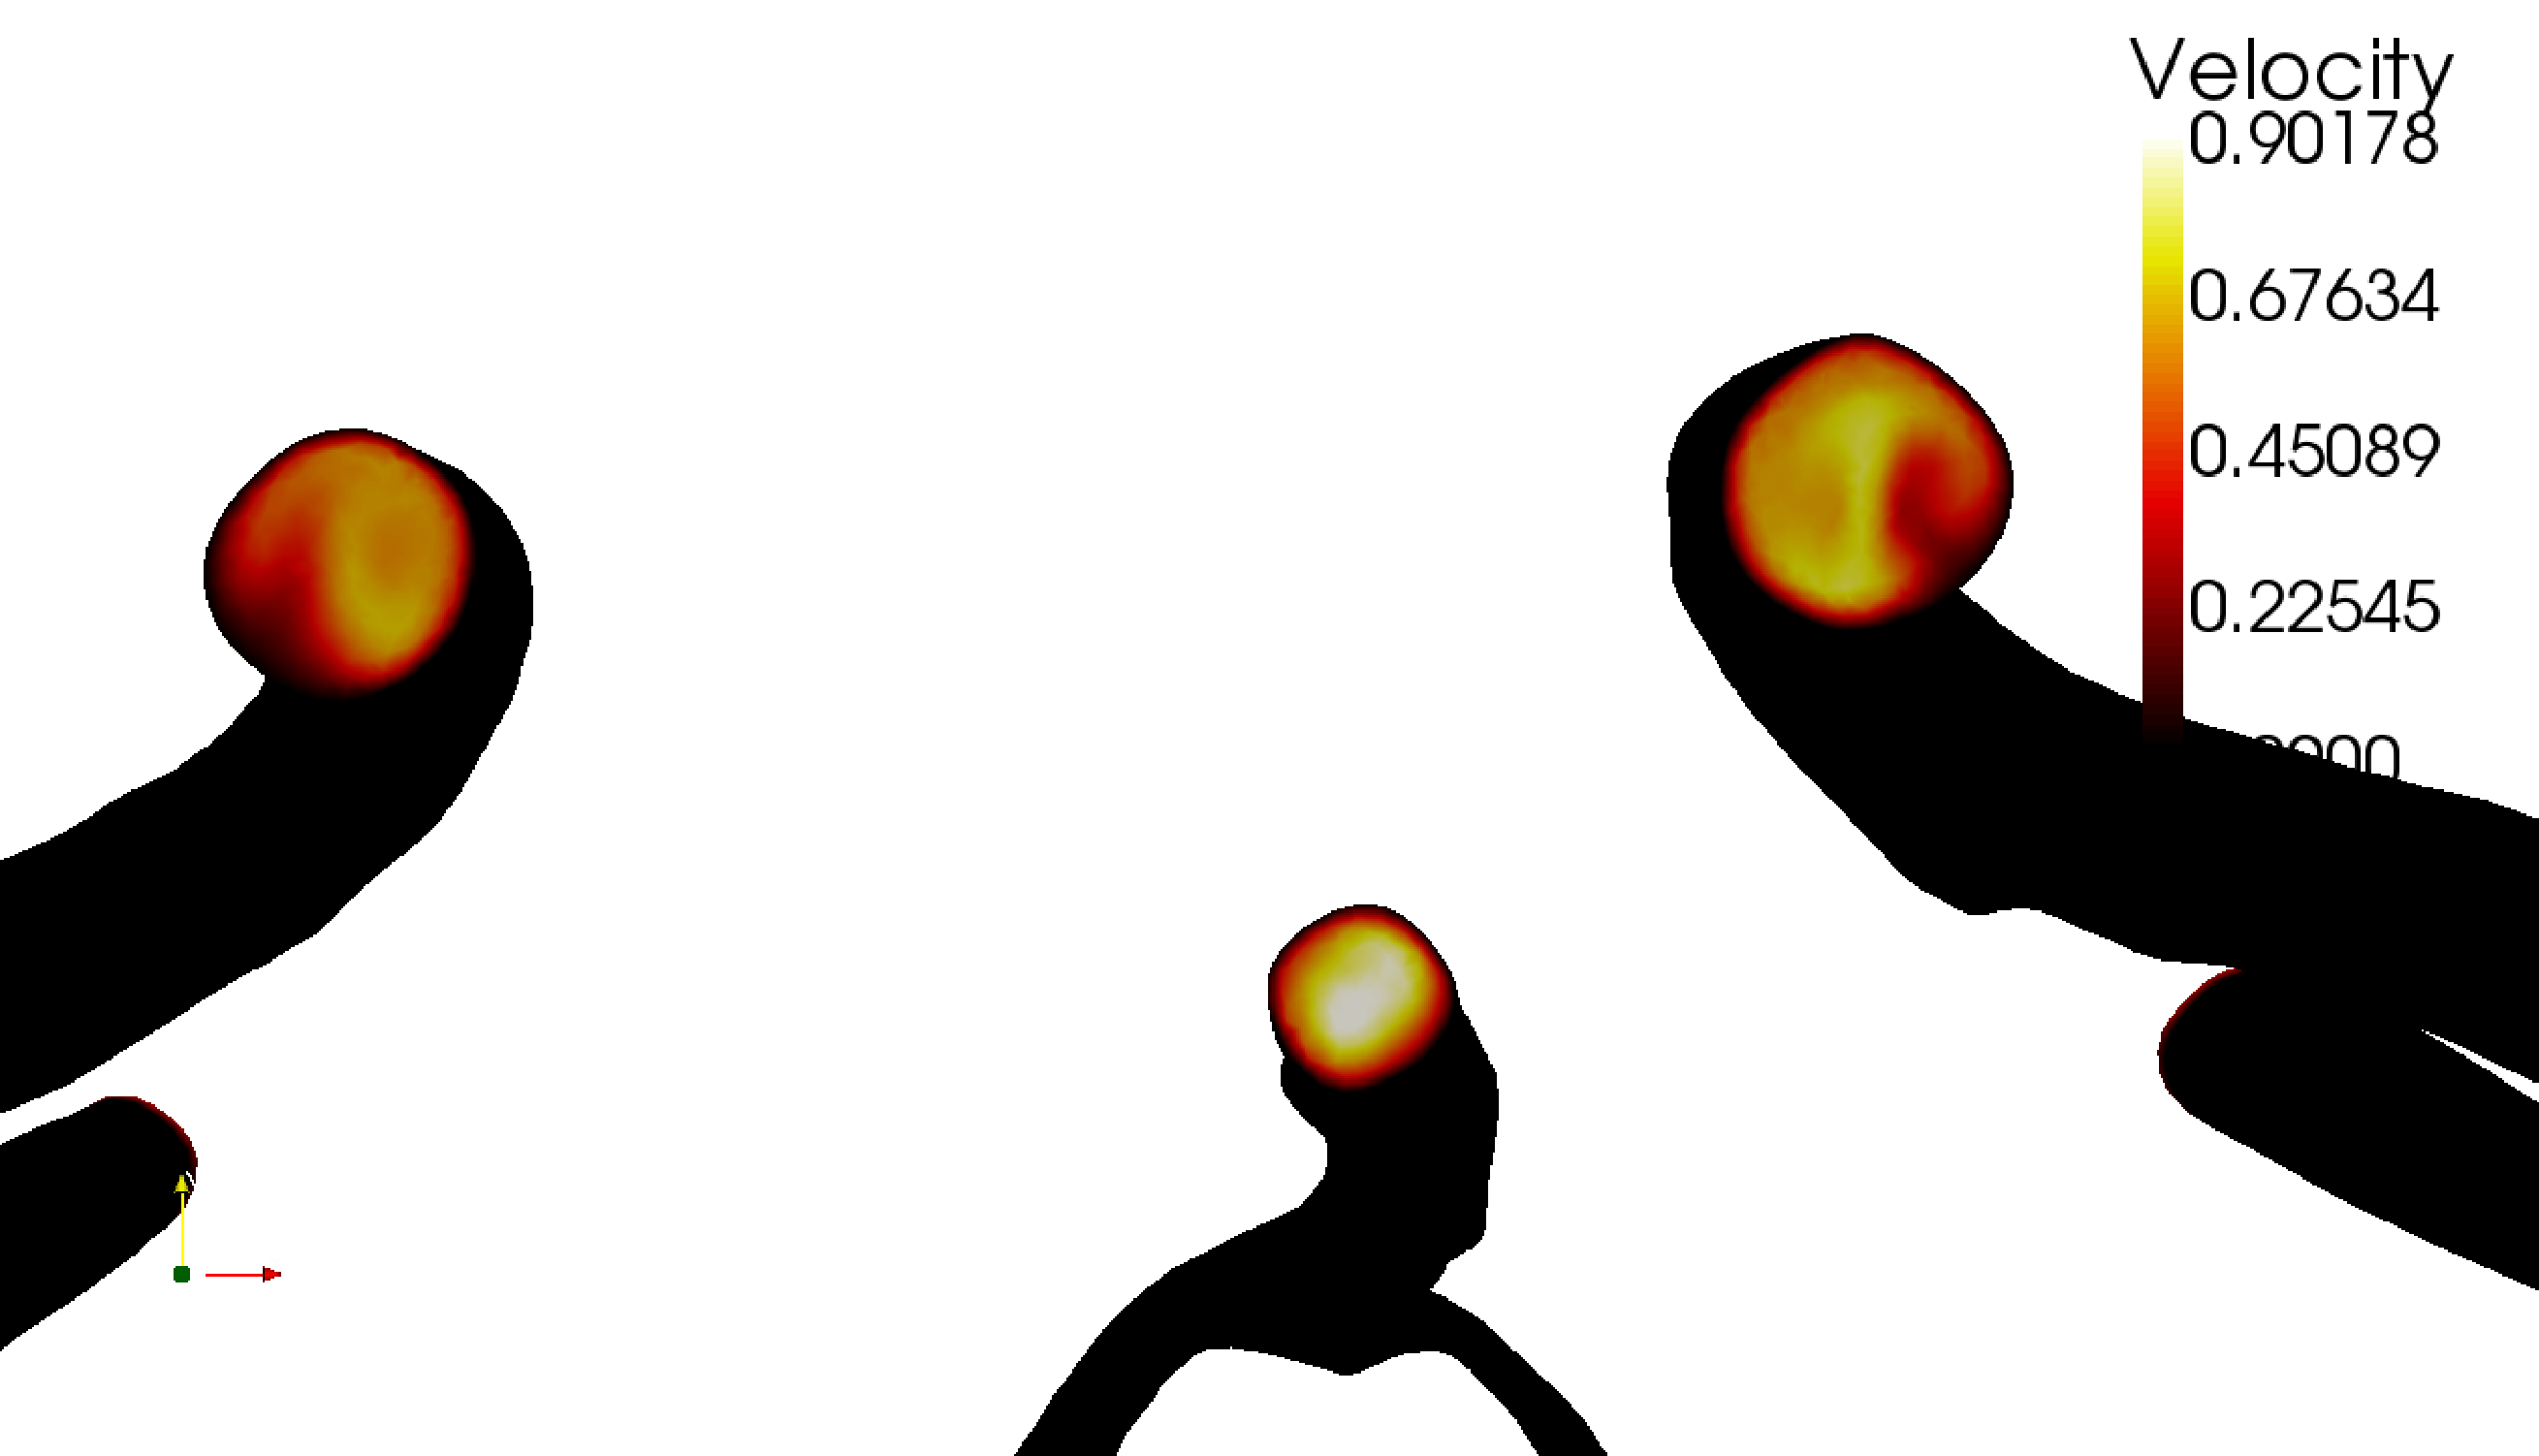
\includegraphics[width=\largefig]{chapters/kvs-2/pdf/cok_ica_vel_peak_syst.pdf}
  \caption{The image on the top shows the plane where the bottom
    image has been cut. The bottom image shows highly
    non-uniform flow in ICA.}
  \label{fig:kvs-2:cok_ica}
\end{figure}
